\documentclass[10pt]{article}
\usepackage[a4paper,margin=28mm]{geometry}
\usepackage[T1]{fontenc}
\usepackage{lmodern}
\usepackage{microtype}
\usepackage{amsmath,amssymb,amsthm}
\usepackage{xcolor}
\usepackage{graphicx}
\usepackage{booktabs}
\usepackage{array}
\usepackage{tabularx}
\usepackage{enumitem}
\usepackage{alltt}
\usepackage{tikz}
\usepackage[colorlinks=true,linkcolor=blue!55!black,citecolor=blue!55!black,urlcolor=blue!55!black]{hyperref}
\hypersetup{bookmarksnumbered=true,pdftitle={An asymptotic formula for clique partitions above the Tur\'an threshold},pdfauthor={Plasma AI}}
\usepackage[capitalise,nameinlink,noabbrev]{cleveref}
\usepackage{xurl}
\def\UrlBreaks{\do\_\do\/\do\.\do\-\do\:}
\def\UrlBigBreaks{}
\Urlmuskip=0mu
\emergencystretch=3em

\newtheorem{theorem}{Theorem}[section]
\newtheorem{lemma}[theorem]{Lemma}
\newtheorem{proposition}[theorem]{Proposition}
\newtheorem{corollary}[theorem]{Corollary}
\theoremstyle{definition}
\newtheorem{definition}[theorem]{Definition}
\theoremstyle{remark}
\newtheorem{remark}[theorem]{Remark}
\numberwithin{equation}{section}

\newcommand{\R}{\mathbb{R}}
\newcommand{\cp}{\operatorname{cp}}
\newcommand{\cps}{\operatorname{cp}^{*}}
\newcommand{\eps}{\varepsilon}
\newcommand{\one}{\mathbf{1}}
\newcommand{\dd}{\mathrm{d}}
\newcommand{\Wm}{\mathcal{W}}
\newcommand{\Hole}{\mathcal{H}}
\newcommand{\lean}[1]{\texttt{#1}}
\newcommand{\leanid}[1]{\expandafter\nolinkurl\expandafter{\detokenize{#1}}}
\newcommand{\Fm}[1]{\cite[#1]{Formalization}}

\newenvironment{leanlisting}{\begin{quote}\footnotesize\begin{alltt}}{\end{alltt}\end{quote}}
\setlist{itemsep=2pt,topsep=4pt}
\renewcommand{\arraystretch}{1.15}

\title{An asymptotic formula for clique partitions above the Tur\'an threshold}
\author{Plasma AI}
\date{November 2026}

\begin{document}
\maketitle

\begin{abstract}
Let $\cp(G)$ be the least number of cliques whose edge sets partition the edges of a graph $G$, single edges counting as cliques, and let $f(n,k)$ be the largest value of $\cp(G)$ over graphs with $n$ vertices and $k$ edges. Erd\H{o}s, Goodman and P\'osa proved $f(n,k)\le\lfloor n^2/4\rfloor$. Erd\H{o}s asked whether this bound can be sharpened when $k>n^2/4$, and Bloom's catalog asks for an estimate of $f(n,k)$ there (Erd\H{o}s Problem~1017). We determine $f(n,k)$ to within $o(n^2)$ at every edge density: $f(n,k)=n^2B(k/n^2)+o(n^2)$ uniformly in $0\le k\le\binom n2$, for an explicit continuous piecewise algebraic function $B$. This provides an asymptotic resolution of Erd\H{o}s Problem~1017, as posed by Erd\H{o}s and as stated by Bloom. Above density $1/4$, $B$ is the larger of two curves built from three families of blow-ups (split, mixed and two-head graphs), each certified by an explicit dual solution. For the upper bound we pass to the fractional relaxation and to limit objects that carry an optimal dual, and we exclude a positive maximum of the difference between the fractional limit and $B$ by a variational argument and a case analysis. The proof is formalized in Lean~4 using Mathlib. This paper proves the shorter parts and one case of the analysis in full; the other parts and cases are proved in full in the Lean development.
\end{abstract}

% ===========================================================================
\section{Introduction}\label{sec:intro}

\subsection{The problem}
All graphs are finite and simple. A \emph{clique partition} of a graph $G$ is a family of cliques of $G$, each with at least two vertices, whose edge sets partition $E(G)$; $\cp(G)$ is the least size of one. For $0\le k\le\binom n2$ put
\[
 f(n,k)=\max\{\cp(G): |V(G)|=n,\ e(G)=k\}.
\]
Single edges are cliques, so $\cp(G)\le e(G)$, with equality when $G$ is triangle-free; taking subgraphs of a complete balanced bipartite graph gives $f(n,k)=k$ for $k\le\lfloor n^2/4\rfloor$. Erd\H{o}s, Goodman and P\'osa~\cite[Theorem~4]{EGP66} proved $f(n,k)\le\lfloor n^2/4\rfloor$ for every $k$, using only edges and triangles; the complete balanced bipartite graph attains the bound. Erd\H{o}s~\cite[item~11, p.~101]{Er71} asked whether it can be sharpened for $k>n^2/4$, noting that ``no satisfactory non-trivial sharpening of our theorem is known''. Bloom~\cite{Bloom} catalogs the question as Erd\H{o}s Problem~1017. Lov\'asz~\cite{Lo68} studied the covering version, in which the cliques need not be edge-disjoint.

\subsection{Previous work}\label{sec:previous}
Write $k=\lfloor n^2/4\rfloor+m$. A maximum family of edge-disjoint triangles together with the remaining edges is a clique partition, so every lower bound on the number of edge-disjoint triangles gives an upper bound on $f$.
\begin{itemize}[leftmargin=1.5em]
\item Gy\H{o}ri's theorems on edge-disjoint triangles and cliques~\cite{Gy88,Gy91} (with a correction in~\cite{Gy92}) give $f(n,k)\le\lfloor n^2/4\rfloor-m$ when $m$ is at most a linear function of $n$ ($m\le2n-10$ for odd $n$ and $m\le3n/2-5$ for even $n$, as stated in~\cite{BLPPPV21,BaWi25}), and $f(n,k)\le\lfloor n^2/4\rfloor-m+O(m^2/n^2)$ when $m=o(n^2)$. A triangle-free graph with $m$ edges placed inside one side of a complete balanced bipartite graph has no $K_4$, and each of its triangles uses one of the added edges, so it needs at least $\lfloor n^2/4\rfloor-m$ cliques; these are the graphs that show the theorem of~\cite{GyKe17} to be sharp. Hence $f(n,k)=\lfloor n^2/4\rfloor-m$ in the first range and $f(n,k)=\lfloor n^2/4\rfloor-m+O(m^2/n^2)$ in the second.
\item Gy\H{o}ri and Keszegh~\cite{GyKe17} proved that every $K_4$-free graph with $\lfloor n^2/4\rfloor+m$ edges has $m$ edge-disjoint triangles; this is sharp for $m$ up to about $n^2/16$, which settles the $K_4$-free case in that range.
\item Kr\'al', Lidick\'y, Martins and Pehova~\cite{KLMP19} bounded decompositions into edges and triangles; their bound implies $f(n,k)\le n^2/4-m/3+o(n^2)$. Blumenthal, Lidick\'y, Pehova, Pfender, Pikhurko and Volec~\cite{BLPPPV21} sharpened it, which gives $f(n,k)\le(n^2-k+2)/3$ for large $n$. Balogh and Wigal~\cite{BaWi25} proved Gy\H{o}ri's conjecture that, for each fixed $r\ge3$, every $n$-vertex graph with $\ell$ edges more than the Tur\'an graph $T_{r-1}(n)$ has $(2-o(1))\ell/r$ edge-disjoint copies of $K_r$ as $n\to\infty$; the case $r=3$ is the result of~\cite{KLMP19}, which they prove again without flag algebras, so for $f$ it gives the same bound.
\item Balogh, He, Krueger, Nguyen and Wigal~\cite{BHKNW26} compared fractional and integral clique decompositions with costs. We use the case $\cp(G)\le\cps(G)+o(n^2)$ of their Theorem~1.10 (\cref{sec:transfer}).
\end{itemize}
A working report on the problem~\cite{EPaD}, which describes itself as AI-generated and not independently verified, computes $f(n,k)$ exactly for $n\le7$ by exhaustive search, records the small-$m$ formula above, and leaves the behavior at positive excess density open. To our knowledge no earlier work determines $f(n,k)$ to within $o(n^2)$ at any fixed density strictly between $1/4$ and $1/2$. This reflects a search, on 3 November 2026, of Bloom's problem entry and its discussion thread, of Formal Conjectures~\cite{FC}, of arXiv, zbMATH Open, Crossref and OpenAlex, and of the web.

\subsection{The main result}
We measure edge density by $d=k/n^2\in[0,1/2]$, not by $k/\binom n2$.

\begin{theorem}[{\leanid{Erdos1017.uniform_asymptotic}}]\label{thm:main}
Let $B\colon[0,1/2]\to\R$ be the continuous function of \cref{def:B}. Then
\begin{equation}\label{eq:main}
 \lim_{n\to\infty}\ \max_{0\le k\le\binom n2}\ \left|\frac{f(n,k)}{n^2}-B\!\left(\frac{k}{n^2}\right)\right|=0 .
\end{equation}
\end{theorem}

\begin{figure}[t]
\centering
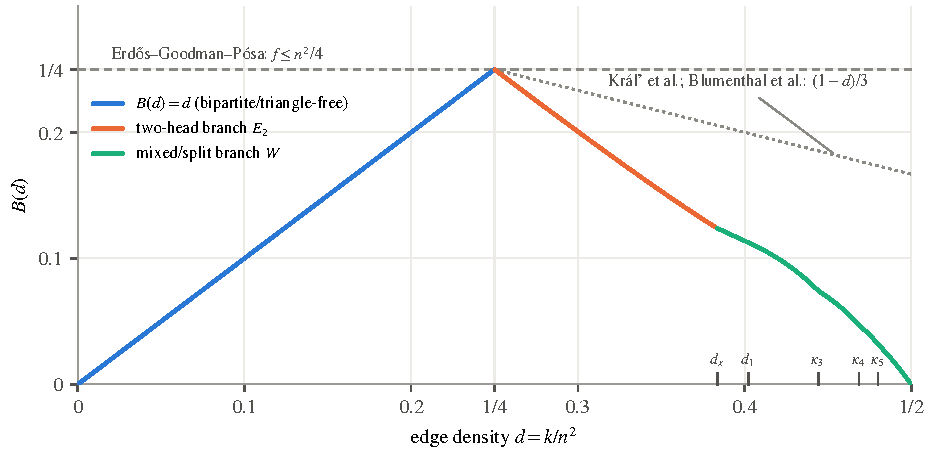
\includegraphics[width=0.92\linewidth]{benchmark.pdf}
\caption{The function $B$, computed numerically from its definition (not checked in Lean). The color shows which family attains $B$. The gray lines are the bound of Erd\H{o}s, Goodman and P\'osa and the normalized bound $(1-d)/3$ of~\cite{KLMP19,BLPPPV21}. Tick marks show the crossing $d_x\approx0.38378$ of the two families, the junction $d_1\approx0.40243$ where the mixed family becomes the split family, and the first kinks $\kappa_3,\kappa_4,\kappa_5$ of the split curve.}
\label{fig:B}
\end{figure}

\Cref{fig:B} shows $B$. It equals $d$ on $[0,1/4]$ and vanishes at $1/2$. On $(1/4,1/2)$ it is the larger of the values of two families of graphs at missing density $\eps=1/2-d$: a \emph{two-head} family $E_2$, which wins on $(1/4,d_x)$, and a \emph{mixed} family $W$, which wins or ties on $(d_x,1/2)$; here $d_x\approx0.38378$ (\cref{sec:branches}). On $[d_1,1/2)$, $d_1=(9\sqrt{21}-1)/100\approx0.40243$, both reduce to split graphs, $B$ is piecewise quadratic in $\sqrt{1-2d}$, and it has kinks at
\[
 \kappa_k=\frac{1-1/k^2}{2}\quad(k\ge3),\qquad B(\kappa_k)=\frac{k-1}{k^3},
\]
which accumulate at $1/2$. \Cref{tab:values} lists some values.

\begin{table}[t]
\centering\small
\begin{tabular}{@{}ccccc@{}}
\toprule
$d$ & $B(d)$ & family attaining $B$ & $\tfrac12-d$ & $(1-d)/3$\\
\midrule
$0.30$ & $0.2007$ & two-head $E_2$ & $0.2000$ & $0.2333$\\
$0.35$ & $0.1533$ & two-head $E_2$ & $0.1500$ & $0.2167$\\
$0.40$ & $0.1139$ & mixed $W$ & $0.1000$ & $0.2000$\\
$0.45$ & $0.0692$ & split (both) & $0.0500$ & $0.1833$\\
\bottomrule
\end{tabular}
\caption{Numerical values of $B$, rounded to four places (not checked in Lean). The column $\tfrac12-d$ is the normalized form of $\lfloor n^2/4\rfloor-m$; the last column is the normalized upper bound of~\cite{KLMP19,BLPPPV21}.}
\label{tab:values}
\end{table}

\begin{remark}[Scope]\label[remark]{rem:scope}
\Cref{thm:main} determines $f(n,k)$ to within $o(n^2)$ at every edge density. This provides an asymptotic resolution of Erd\H{o}s Problem~1017, as posed by Erd\H{o}s and as stated by Bloom. For $k>n^2/4$ the bound $\lfloor n^2/4\rfloor$ is replaced by $n^2B(k/n^2)+o(n^2)$, and the lower bound of \cref{prop:lower} shows that this leading term is exact. At every fixed density $d>1/4$ the new bound is smaller by a positive multiple of $n^2$, because $B(d)\le(1-d)/3<1/4$; this inequality follows from \cref{thm:main} and the bound of~\cite{BLPPPV21}, and is not checked in Lean. Lower-order terms and the regime near density $1/2$ are discussed in \cref{sec:discussion}.
\end{remark}

\subsection{Method}
The proof uses linear-programming duality for clique decompositions, as in~\cite{BHKNW26} and in the concurrent work~\cite{Zh26}; limit objects of graphs, decorated with an optimal dual charge on pairs; first and second variations of an extremal limit object under reweighting of its vertex measure; a spectral condition on a shifted charge kernel; and a case analysis of where a positive maximum of $F-B$ can sit. To our knowledge, the formula for $B$, the use of the two-head and mixed families with their dual certificates to define it above density $1/4$, and the matching upper bound are new; this rests on the literature search described in \cref{sec:previous}.

Three ingredients come from elsewhere. (i) The transfer $\cp(G)\le\cps(G)+o(n^2)$ is the case $t=2$, unit costs, of~\cite[Theorem~1.10]{BHKNW26}; the Lean development proves this case again rather than assuming it (\leanid{exists_same_graph_integer_upper_transfer}). (ii) The compactness of graph limits is the Lov\'asz--Szegedy compactness theorem~\cite{LS07}; the development adapts Cameron Freer's Lean formalization of it~\cite{Freer} to countable families of graphons with one common subsequence (\leanid{Erdos1017.GraphonFamily.compact_countable}). (iii) The Lean proof of the transfer uses Szemer\'edi's regularity lemma as formalized in Mathlib~\cite{Mathlib} and a nibble argument in the spirit of~\cite{FR85,PS89}. We do not use the packing bounds of~\cite{KLMP19,BLPPPV21,BaWi25}. Numerical evaluation indicates that $B(d)$ lies strictly below their bound $(1-d)/3$ for $1/4<d\le1/2$ (\cref{tab:values}); this strict comparison is not proved here and is not checked in Lean.

\subsection{The formal proof and the plan of this paper}
The proof is formalized in Lean~4 using Mathlib; the source code is available in~\cite{Formalization} (\cref{sec:lean}). Its statement, the theorem \leanid{Erdos1017.uniform_asymptotic}, is given in a file that imports only Mathlib and copies the definitions of clique edge partitions and of $f$ verbatim from Formal Conjectures~\cite{FC}; its axioms are \lean{propext}, \lean{Classical.choice} and \lean{Quot.sound}. We regard the Lean development as the proof of record. No complete human-readable proof of $F\le B$ exists yet: this paper proves one of the five exclusions in full, the blueprint summarizes the others, and the Lean development is the only complete proof. Its blueprint follows it in prose, module by module, proving some steps and cases in full and summarizing the others. The blueprint has four files in the repository~\cite{Formalization}: \lean{blueprint/proof.md} (sections 0 to 7 and 9), \lean{blueprint/selected\_model.md} (section 8), \lean{blueprint/exclusions.md} (section 10) and \lean{blueprint/certificates.md} (section 11). We cite it by section, as in~\Fm{\S10.2}.

This paper gives complete proofs of the fractional limit (\cref{sec:limit}); of the lower bound and the properties of $B$, except the branch facts of \cref{sec:branches}, which are proved in Lean (\cref{sec:benchmark}); of the reduction to the inequality $F\le B$ (\cref{sec:transfer}); of \cref{lem:posmax}; and of \cref{thm:location} from the stated inputs \cref{prop:strict}, \cref{thm:selected}, the branch facts of \cref{sec:branches} and \cref{thm:smoothW}. It proves one of the five final exclusions, \cref{thm:lowerE2}, in full from structural facts that it states precisely, and it summarizes the others. The integer transfer is quoted from~\cite{BHKNW26} (\cref{thm:transfer}). The limit models and their selection, the structure of the selected model and the remaining exclusions are proved in full only in Lean; the blueprint follows these proofs in prose. \Cref{fig:tree} shows how the parts fit together.

\begin{figure}[t]
\centering
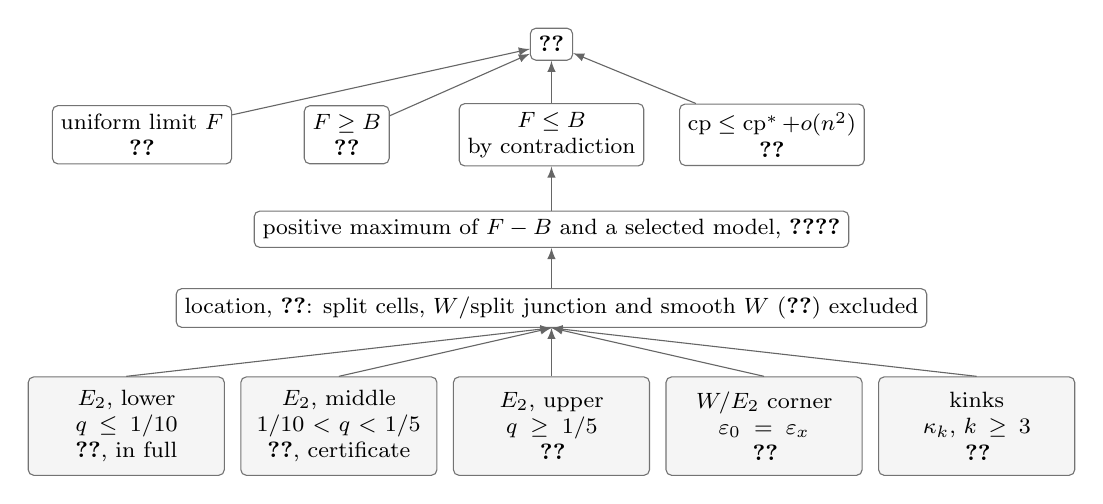
\begin{tikzpicture}[
  box/.style={draw=black!55, rounded corners=2pt, align=center, font=\footnotesize, inner sep=3pt, fill=white},
  leaf/.style={draw=black!55, rounded corners=2pt, align=center, font=\footnotesize, inner sep=2pt, fill=black!4, text width=2.35cm, minimum height=1.25cm},
  arr/.style={-latex, black!60}]
\node[box] (main) at (0,0) {\cref{thm:main}};
\node[box] (lim) at (-5.2,-1.15) {uniform limit $F$\\ \cref{sec:limit}};
\node[box] (low) at (-2.6,-1.15) {$F\ge B$\\ \cref{sec:benchmark}};
\node[box] (up) at (0,-1.15) {$F\le B$\\ by contradiction};
\node[box] (tr) at (2.8,-1.15) {$\cp\le\cps+o(n^2)$\\ \cref{sec:transfer}};
\node[box] (sel) at (0,-2.35) {positive maximum of $F-B$ and a selected model, \cref{sec:models,sec:structure}};
\node[box] (loc) at (0,-3.35) {location, \cref{sec:location}: split cells, $W$/split junction and smooth $W$ (\cref{sec:smoothW}) excluded};
\node[leaf] (l1) at (-5.4,-4.85) {$E_2$, lower\\ $q\le1/10$\\ \cref{sec:lowerE2}, in full};
\node[leaf] (l2) at (-2.7,-4.85) {$E_2$, middle\\ $1/10<q<1/5$\\ \cref{sec:middleE2}, certificate};
\node[leaf] (l3) at (0,-4.85) {$E_2$, upper\\ $q\ge1/5$\\ \cref{sec:upperE2}};
\node[leaf] (l4) at (2.7,-4.85) {$W/E_2$ corner\\ $\eps_0=\eps_x$\\ \cref{sec:corner}};
\node[leaf] (l5) at (5.4,-4.85) {kinks\\ $\kappa_k$, $k\ge3$\\ \cref{sec:cusps}};
\foreach \x in {lim,low,up,tr} \draw[arr] (\x) -- (main);
\draw[arr] (sel) -- (up);
\draw[arr] (loc) -- (sel);
\foreach \x in {l1,l2,l3,l4,l5} \draw[arr] (\x.north) -- (loc.south);
\end{tikzpicture}
\caption{Structure of the proof. Arrows point from a part to the statement it supports. The upper bound $F\le B$ is proved by contradiction: the five leaves exclude every location of a positive maximum of $F-B$ that survives \cref{sec:location}.}
\label{fig:tree}
\end{figure}

% ===========================================================================
\section{The fractional relaxation and its limit}\label{sec:limit}

The \emph{fractional clique partition number} $\cps(G)$ is the minimum of $\sum_Qx_Q$ over weights $x\ge0$ on cliques $Q$ of $G$ with at least two vertices such that $\sum_{Q\ni e}x_Q=1$ for every edge $e$. Its dual maximizes $\sum_ey_e$ over real weights $y$ on edges subject to
\begin{equation}\label{eq:dualfeas}
 \sum_{e\subseteq Q}y_e\le1\qquad\text{for every clique }Q\text{ of }G.
\end{equation}
Thus every $y$ satisfying \eqref{eq:dualfeas} gives $\cp(G)\ge\cps(G)\ge\sum_ey_e$. Let $f^*(n,k)$ be the maximum of $\cps(G)$ over graphs with $n$ vertices and $k$ edges; then $f^*\le f$.

\begin{lemma}[Edits and blow-ups]\label[lemma]{lem:edit}
Adding an edge raises $\cps$ by at most $1$, and deleting an edge raises it by at most $3$. Consequently, if $0\le k_1\le k_2\le\binom n2$, then $-3(k_2-k_1)\le f^*(n,k_2)-f^*(n,k_1)\le k_2-k_1$. If $\Gamma[t]$ replaces each vertex of a graph $\Gamma$ by $t$ independent copies, then $e(\Gamma[t])=t^2e(\Gamma)$ and $\cps(\Gamma[t])=t^2\cps(\Gamma)$; isolated vertices do not change $\cps$.
\end{lemma}

\begin{proof}
An added edge can be covered by itself. To delete an edge $xy$, replace each clique $Q\ni xy$ of weight $x_Q$ by the following fractional partition of the edges of $Q$ other than $xy$: choose one of $x,y$ uniformly, keep every other vertex of $Q$ independently with probability $1/2$, and give each outcome with at least two vertices weight $4x_Q$ times its probability. Every edge of $Q$ other than $xy$ survives with probability $1/4$, so it receives weight exactly $x_Q$, and $xy$ never survives. The cliques through $xy$ have total weight $1$, so the cost rises by at most $3$. In the other direction, deleting an edge lowers $\cps$ by at most $1$ (adding it back raises $\cps$ by at most $1$), and adding an edge lowers it by at most $3$ (deleting it again raises $\cps$ by at most $3$). For the upper inequality delete $k_2-k_1$ edges from an extremal graph with $k_2$ edges; for the lower one add $k_2-k_1$ edges to an extremal graph with $k_1$ edges. For blow-ups, give each of the $t^{|Q|}$ lifts of $Q$ weight $t^{2-|Q|}x_Q$; conversely every clique of $\Gamma[t]$ meets each class of copies at most once and projects to a clique of $\Gamma$, so aggregating a partition of $\Gamma[t]$ by projection and dividing by $t^2$ gives a partition of $\Gamma$.
\end{proof}

In Lean these are \leanid{FractionalGraph.value_add_edge_le}, \leanid{FractionalGraph.value_delete_edge_le}, \leanid{extremal_edit_bounds} and \leanid{value_blowup}~\Fm{\S3}. The constants $1$ and $3$ reappear as the charge range $[-3,1]$ in \cref{sec:models}. Following Lean, we define the limit function as a penalized supremum and prove that it is a limit.

\begin{definition}\label[definition]{def:F}
For $d\in[0,1/2]$ let $F(d)$ be the supremum of $0$ and of the numbers $\cps(G)/N^2-3\,|e(G)/N^2-d|$ over all graphs $G$ on $N\ge1$ vertices (\leanid{FractionalGraph.densityLimit}).
\end{definition}

\begin{theorem}\label{thm:limit}
\textup{(a)} $F$ is $3$-Lipschitz on $[0,1/2]$. \textup{(b)} If $k_n\le\binom n2$ and $k_n/n^2\to d$, then $f^*(n,k_n)/n^2\to F(d)$. \textup{(c)} $\max_{0\le k\le\binom n2}|f^*(n,k)/n^2-F(k/n^2)|\to0$. \textup{(d)} $F(d)=d$ for $d\le1/4$ and $F(1/2)=0$.
\end{theorem}

\begin{proof}
(a) Each candidate in \cref{def:F} is a $3$-Lipschitz function of $d$, and all are at most $1/2$; a bounded supremum of $3$-Lipschitz functions is $3$-Lipschitz.

(b) Let $G_n$ be extremal with $k_n$ edges. Its candidate gives $f^*(n,k_n)/n^2\le F(d)+3|k_n/n^2-d|$, so $\limsup f^*(n,k_n)/n^2\le F(d)$. Conversely fix a graph $G$ on $N$ vertices. For large $n$ let $t=\lfloor n/N\rfloor$ and take $G[t]$ plus $n-tN$ isolated vertices; it has $t^2e(G)$ edges and $\cps=t^2\cps(G)$ by \cref{lem:edit}. Edit it to exactly $k_n$ edges, which is possible since $k_n\le\binom n2$; each edit lowers $\cps$ by at most $3$. Dividing by $n^2$ and letting $n\to\infty$ with $G$ fixed gives $\liminf f^*(n,k_n)/n^2\ge\cps(G)/N^2-3|e(G)/N^2-d|$. Taking the supremum over $G$ (and noting $f^*\ge0$) gives $\liminf\ge F(d)$.

(c) Otherwise there are $\eta>0$, $n_i\to\infty$ and $k_i$ with $|f^*(n_i,k_i)/n_i^2-F(k_i/n_i^2)|\ge\eta$. Pass to a subsequence with $k_i/n_i^2\to d$, extend $(k_i)$ to a sequence defined for all $n$ with $k_n/n^2\to d$, and apply (b) and the continuity of $F$.

(d) For $k\le\lfloor n^2/4\rfloor$ a $k$-edge subgraph of a complete balanced bipartite graph has only edges as cliques, so $f^*(n,k)=k$; apply (b) with $k_n=\lfloor dn^2\rfloor$. At $d=1/2$ take $k_n=\binom n2$: $\cps(K_n)=1$.
\end{proof}

In Lean: \leanid{densityLimit_lipschitz}, \leanid{tendsto_extremal_of_density}, \leanid{extremal_uniform_convergence}, \leanid{densityLimit_eq_self}, \leanid{densityLimit_half}~\Fm{\S3--4}.

% ===========================================================================
\section{The benchmark and the lower bound}\label{sec:benchmark}

\subsection{Weighted blow-ups}
Let $\Gamma$ be a graph on $\{1,\dots,s\}$, $w$ a probability vector and $y$ a real weight on $E(\Gamma)$ satisfying \eqref{eq:dualfeas} for every clique of $\Gamma$. Put $D(\Gamma,w)=\sum_{ij\in E(\Gamma)}w_iw_j$ and $\Phi(\Gamma,w,y)=\sum_{ij\in E(\Gamma)}y_{ij}w_iw_j$.

\begin{lemma}\label[lemma]{lem:blowup}
$F(D(\Gamma,w))\ge\Phi(\Gamma,w,y)$.
\end{lemma}

\begin{proof}
For rational $w_i=m_i/M$ let $G$ replace vertex $i$ by $m_i$ independent copies. A clique of $G$ meets each class at most once and projects to a clique of $\Gamma$, so the pull-back of $y$ satisfies \eqref{eq:dualfeas} on $G$, and $\cps(G)\ge\Phi(\Gamma,w,y)M^2$. Since $e(G)/M^2=D(\Gamma,w)$, the candidate of $G$ in \cref{def:F} has no penalty. For real $w$ approximate by rational vectors and use the continuity of $F$ and of the two quadratic forms.
\end{proof}

\subsection{Three families and where $B$ comes from}\label{sec:families}
Each base graph below has a \emph{tail} of $N$ vertices forming a clique, with total weight $u$ spread equally; as $N\to\infty$ the blow-up of the tail approaches a clique on $un$ vertices, and by \cref{lem:blowup} and continuity of $F$ we may pass to the limit. Write $J=j(j+1)$ for an integer $j\ge1$.

\emph{Split base.} One \emph{head} of weight $a$ joined to the tail ($u=1-a$). Charges: $2/(j+1)$ on head--tail edges, $-2/J$ on tail--tail edges. A clique with the head and $i$ tail vertices has charge $i(2j+1-i)/J\le1$, because $J-i(2j+1-i)=(i-j)(i-j-1)\ge0$ for every integer $i$; a clique without the head has negative charge. In the limit the blow-up is the split graph $I_a\vee K_{1-a}$ (an independent set of $an$ vertices joined to a clique of $(1-a)n$ vertices), of missing density $\eps=a^2/2$, and \cref{lem:blowup} gives
\begin{equation}\label{eq:splitlower}
 F\bigl(\tfrac{1-a^2}2\bigr)\ \ge\ H_j(a):=\frac{2ja(1-a)-(1-a)^2}{J}=\frac{-(2j+1)a^2+2(j+1)a-1}{j(j+1)}.
\end{equation}
The tight cliques are those with one head vertex and $j$ or $j+1$ tail vertices. The best $j$ for given $a$ follows from
\[
 H_{j+1}(a)-H_j(a)=\frac{2(a-1)\bigl((j+1)a-1\bigr)}{j(j+1)(j+2)},
\]
which is positive exactly when $(j+1)a<1$; so the best choice is $j(a)=\max(1,\lceil(1-a)/a\rceil)$. At $a=1/k$ the choices $j=k-1$ and $j=k$ tie, which produces the kinks $\kappa_k$.

\emph{Leaf base (mixed family).} A \emph{leaf} $v_a$ of weight $a$, a head $v_b$ of weight $b$ and the tail; edges $v_av_b$, $v_b$--tail and tail--tail ($v_a$ is not joined to the tail). Charges: $1$ on $v_av_b$ and the split charges on $v_b$ and the tail. A clique containing $v_a$ is the edge $v_av_b$; every other clique was checked above. The limit blow-up is $(I_a\sqcup K_u)\vee I_b$, with missing density $(a^2+b^2)/2+au$ and dual value $ab+\frac{2}{j+1}bu-\frac{u^2}{J}$.

\emph{Two-head base.} Two heads $v_\alpha,v_\beta$ of weights $\alpha,\beta$ and the tail, all joined. Charges $1$ on $v_\alpha v_\beta$, $2/3$ on $v_\alpha$--tail, $-2/3$ on $v_\beta$--tail, $-1/3$ on tail--tail. A clique with $v_\alpha$ and $i$ tail vertices has charge $i(5-i)/6\le1$ (the case $j=2$ above); with both heads and $i$ tail vertices, $1-i(i-1)/6\le1$; without $v_\alpha$, at most $0$. The limit blow-up is the complete multipartite graph $K_{\alpha n,\beta n,1^{un}}$, with missing density $(\alpha^2+\beta^2)/2$ and dual value $\alpha\beta+\frac23(\alpha-\beta)u-\frac{u^2}6$.

For the last two families, fixing the missing density leaves one free part size. The branches of $B$ are the dual values at the critical points along these level sets: a direct computation shows that at the points
\begin{align}
 (a,b,u)&=\frac{(-3s^2+3s+1,\ 4s+1,\ s(4s+1))}{s^2+8s+2}\qquad(\sigma_d\le s\le\sigma_0;\ j=2),\label{eq:mixedpts}\\
 (\alpha,\beta,u)&=\Bigl(\frac{z(5z-3)}{4\rho(z)},\ \frac{z(1-z)}{4\rho(z)},\ \frac{3z-2}{2\rho(z)}\Bigr)\qquad(2/3\le z\le z_c),\label{eq:twoheadpts}
\end{align}
with $\rho(z)=z^2+z-1$, the gradient of the dual value is a combination of the gradients of $a+b+u$ and of the missing density (a polynomial identity in $s$, respectively $z$; not checked in Lean). The missing densities and dual values at these points are the rational functions $E(s),C_W(s)$ and $\eps_2(z),C_2(z)$ of \cref{def:B} (\leanid{mixed_parameter_lower}, \leanid{twoHead_parameter_lower}). The constants mark transitions between families:
\begin{itemize}[leftmargin=1.5em]
\item $\sigma_0=(3+\sqrt{21})/6$ is the positive root of $3s^2-3s-1$, where the leaf weight $a$ in \eqref{eq:mixedpts} vanishes. There the mixed family becomes the split family with $j=2$; this is the $W$/split junction $\eps_*=E(\sigma_0)$.
\item $\sigma_d$ is where the mixed value equals the missing density, $C_W(\sigma_d)=E(\sigma_d)$. For $\eps\ge\eps_d$ the leaf base with $j=1$, $b=1/2$, $u=\sqrt{1/2-2\eps}$ and $a=1/2-u$ has dual value exactly $\eps$, and $W$ continues as $W(\eps)=\eps$.
\item $z=2/3$ gives $u=0$, $\alpha=\beta=1/2$: the balanced complete bipartite graph at $\eps=1/4$. At $z_c$ the two-head value meets the split value $H_2(\sqrt{2\eps})$ (\cref{lem:welldefined}); for smaller $\eps$, $E_2$ follows the split curve.
\end{itemize}
The parameter $q=3z-2$ used below determines the tail weight by $u=9q/(2R(q))$, with $R$ as in \eqref{eq:qparam}.

As a heuristic for the choice of families: every family above is a blow-up of a small graph, so its value is the value of a finite linear program, and complete multipartite graphs with a clique part are the natural candidates; indeed no complete multipartite profile, with countably many parts and a clique remainder, exceeds $B$ at its own density (\leanid{MultipartiteCountableDual.normalized_value_le_benchmark};~\Fm{\S7}). Starting from the balanced complete bipartite graph, the two-head family adds edges by growing a clique tail while keeping two large independent heads, until $E_2$ switches to the split family, the extreme case with one head. The mixed family adds a leaf joined only to the head: each leaf edge carries the largest possible charge $1$, while the missing pairs between the leaf and the tail lower the density. The derivation above explains the shape of $B$; the proofs use only the explicit charges and part sizes. We do not claim that the critical points are global maxima of the dual value on the level sets, and we do not identify the multipartite optimum.

\subsection{Definition of $B$}
\begin{definition}\label[definition]{def:B}
For $0<a\le1$ let $j(a)=\max(1,\lceil(1-a)/a\rceil)$ and $H(a)=H_{j(a)}(a)$, with $H_j$ as in \eqref{eq:splitlower}; $H(0)=0$. Let $\sigma_0=(3+\sqrt{21})/6$, $\eps_*=(51-9\sqrt{21})/100$, $Q(\sigma)=\sigma^2+8\sigma+2$,
\[
 E(\sigma)=\frac{2+16\sigma+33\sigma^2-15\sigma^4}{2Q(\sigma)^2},\qquad
 C_W(\sigma)=\frac{6+46\sigma+85\sigma^2-16\sigma^3-16\sigma^4}{6Q(\sigma)^2},
\]
$\sigma_d$ the root in $[1,11/10]$ of $29\sigma^3-16\sigma^2-14\sigma-2$, $\eps_d=E(\sigma_d)$, and $\sigma_W$ the inverse of $E$ on $[\eps_*,\eps_d]$. Let
\[
 W(\eps)=H(\sqrt{2\eps})\ (0\le\eps\le\eps_*),\qquad C_W(\sigma_W(\eps))\ (\eps_*\le\eps\le\eps_d),\qquad \eps\ (\eps_d\le\eps\le1/4).
\]
For $2/3\le z\le4/5$ let $\rho(z)=z^2+z-1$,
\[
 \eps_2(z)=\frac{z^2(13z^2-16z+5)}{16\rho(z)^2},\qquad
 C_2(z)=\eps_2(z)+\frac{(3z-2)^2(1-z)(3z-1)}{24\rho(z)^2},
\]
$z_c$ the root in $[3/4,4/5]$ of $-95z^4+18z^3+193z^2-168z+40$, $\eps_c=\eps_2(z_c)$, and $z_2$ the inverse of $\eps_2$ on $[\eps_c,1/4]$. Let $E_2(0)=0$,
\[
 E_2(\eps)=H(\sqrt{2\eps})\ (0<\eps\le\eps_c),\qquad C_2(z_2(\eps))\ (\eps_c\le\eps\le1/4).
\]
Finally $B(d)=d$ for $0\le d\le1/4$, $B(d)=\max\{W(1/2-d),E_2(1/2-d)\}$ for $1/4<d<1/2$, and $B(1/2)=0$.
\end{definition}

No decimal value enters the definition. The Lean statement defines $\sigma_d$, $z_c$ and the two inverses as infima of their exact solution sets in the stated intervals (\cref{sec:lean}).

\begin{lemma}\label[lemma]{lem:welldefined}
The roots $\sigma_d$ and $z_c$ exist and are unique, the inverses are well defined and continuous, the pieces of $W$ and $E_2$ agree at their breakpoints, and $B$ is continuous on $[0,1/2]$.
\end{lemma}

\begin{proof}
We have
\[
 E'(\sigma)=-\frac{\sigma(2+24\sigma+93\sigma^2+120\sigma^3)}{Q(\sigma)^3}<0,\qquad
 \eps_2'(z)=\frac{z(21z^3-39z^2+24z-5)}{8\rho(z)^3}<0
\]
on $[1,\sigma_0]$ and $[2/3,4/5]$; for the second, $\rho>0$ there, and the cubic in the numerator has derivative $3(3z-2)(7z-4)\ge0$ and value $-1/125$ at $4/5$. Moreover $E(\sigma_0)=\eps_*$ and $E(1)=18/121$, and $\eps_2$ decreases from $1/4$ to $13/121$. A continuous strictly monotone function on an interval has a continuous inverse, so $\sigma_W$ and $z_2$ are well defined and continuous. The cubic defining $\sigma_d$ equals $29(\sigma-1)^3+71(\sigma-1)^2+41(\sigma-1)-3$, so it increases on $[1,\infty)$ and changes sign on $[1,11/10]$; the quartic defining $z_c$ equals $\frac{25}{256}-\frac{135}{16}t-\frac{697}{8}t^2-267t^3-95t^4$ with $t=z-3/4$, so it decreases on $[3/4,\infty)$ and changes sign on $[3/4,4/5]$. At $\eps_*$ one checks $\sqrt{2\eps_*}=(9-\sqrt{21})/10=:a_*$ and $C_W(\sigma_0)=H_2(a_*)$; here $j(a_*)=2$ because $(1-a_*)/a_*=\sigma_0\in(1,2)$. At $\eps_d$,
\[
 C_W(\sigma)-E(\sigma)=\frac{\sigma(29\sigma^3-16\sigma^2-14\sigma-2)}{6Q(\sigma)^2}=0.
\]
At $z_c$ the identity
\[
 \Bigl(C_2(z)+\tfrac53\eps_2(z)+\tfrac16\Bigr)^2-2\eps_2(z)=\frac{z^2(z-1)^2(-95z^4+18z^3+193z^2-168z+40)}{576\,\rho(z)^4}
\]
gives $C_2(z_c)=H_2(\sqrt{2\eps_c})$, the relevant square root being positive; here $j(\sqrt{2\eps_c})=2$ because $\eps_c\in(1/10,9/80)$ (\cref{sec:branches}). Each $H_j$ is continuous and adjacent formulas agree at $a=1/(j+1)$, and $H(a)\to0$ as $a\to0$. At $d=1/4$: $W(1/4)=1/4=C_2(2/3)=E_2(1/4)$.
\end{proof}

In Lean: \leanid{sigmaD_spec}, \leanid{zC_spec}, \leanid{mixedInverse_spec}, \leanid{twoHeadInverse_spec}, \leanid{mixed_branch_match}, \leanid{twoHead_branch_match}, \leanid{benchmark_continuousOn}~\Fm{\S2}.

\subsection{Branch structure}\label{sec:branches}
The following facts about $B$ alone are proved in Lean~\Fm{\S2}. The constants are ordered
\[
 \eps_*<\tfrac1{10}<\eps_c<\tfrac9{80}<\eps_x<\tfrac18<\eps_d<\tfrac14,
\]
where on $[\eps_c,\eps_d]$ the two curves cross exactly once, at $\eps_x$ with $23243416<2\cdot10^8\eps_x<23243417$ (\leanid{exists_unique_crossing_on_overlap}; the other inequalities are \leanid{epsilonStar_lt_tenth}, \leanid{tenth_lt_epsilonC}, \leanid{epsilonC_lt_nine_eightieths}, \leanid{eighth_lt_epsilonD} and \leanid{epsilonD_lt_quarter}). For $\eps_*<\eps<1/4$, either $W$ strictly wins (and then $\eps<\eps_d$), or $E_2$ strictly wins (and then $\eps>\eps_c$), or the two are equal (and then $\eps_c<\eps<\eps_d$; \leanid{family_contact_alternatives}). Hence the continuous function $E_2-W$ vanishes on $(\eps_*,1/4)$ only at $\eps_x$, is negative on $(\eps_*,\eps_c]$ and is positive on $[\eps_d,1/4)$; so $W$ strictly wins on $(\eps_*,\eps_x)$ and $E_2$ strictly wins on $(\eps_x,1/4)$. With $d_x=1/2-\eps_x\approx0.38378$ and $d_1=1/2-\eps_*$, $B$ is therefore given by the curved part of $E_2$ on $(1/4,d_x)$, by the curved part of $W$ on $(d_x,d_1)$, and, since $W$ and $E_2$ both equal $H(\sqrt{2\eps})$ for $\eps\le\eps_*$, by the split value $H(\sqrt{1-2d})$ on $[d_1,1/2)$. On the two-head branch we use $q=3z-2$ and
\begin{equation}\label{eq:qparam}
 R(q)=1+7q+q^2,\quad \ell(q)=\frac{2-q}{2+q},\quad h(q)=\frac{(q+2)^2(1+4q+13q^2)}{8R(q)^2},\quad g(q)=\frac{q(1+2q)}{2R(q)} .
\end{equation}
Where $E_2$ strictly wins there is $q\in(0,213/1000)$ with $d=(1-h(q))/2$, $B(d)=C_2((q+2)/3)$ and $B'(d)=-\ell(q)$ (\leanid{strict_twoHead_contact_parameters}). Numerically (not checked in Lean), $d\approx0.3558$, $0.3821$, $0.3838$ for $q=1/10$, $1/5$, $213/1000$. Where $W$ strictly wins, $B'(d)=-(s+1)/(3s)$ at $s=\sigma_W(1/2-d)$ (\leanid{benchmark_mixed_hasDerivAt_strict}). At a kink, $B(\kappa_k)=(k-1)/k^3$ (\leanid{splitValue_reciprocal}). Finally, $B(d)\ge1/2-d$ on $[1/4,1/2]$, from the two-head family for $d\le3/8$ and the split family above (\leanid{benchmark_ge_missing},~\Fm{\S8.3}).

\subsection{The lower bound}

\begin{proposition}\label[proposition]{prop:lower}
$F\ge B$ on $[0,1/2]$. Consequently, for every $\eta>0$ there is $N$ such that $f(n,k)>n^2(B(k/n^2)-\eta)$ for all $n\ge N$ and $0\le k\le\binom n2$.
\end{proposition}

\begin{proof}
For $d\le1/4$ use \cref{thm:limit}(d). For $1/4<d<1/2$ we show $F(1/2-\eps)\ge W(\eps)$ and $F(1/2-\eps)\ge E_2(\eps)$. On the split pieces apply \eqref{eq:splitlower} with $a=\sqrt{2\eps}$ and $j=j(a)$. On $[\eps_*,\eps_d]$ apply the leaf base with $j=2$ at the points \eqref{eq:mixedpts}: they are nonnegative because $s\le\sigma_0$, sum to $1$, and give missing density $E(s)$ and value $C_W(s)$ (polynomial identities in $s$). On $[\eps_d,1/4]$ use the leaf base with $j=1$ as above; its weights are nonnegative because $\eps_d>1/8$. On $[\eps_c,1/4]$ apply the two-head base at the points \eqref{eq:twoheadpts}, which give missing density $\eps_2(z)$ and value $C_2(z)$. The second statement follows from $F\ge B$, $f\ge f^*$ and \cref{thm:limit}(c).
\end{proof}

In Lean: \leanid{split_charge_le_one}, \leanid{leaf_charge_le_one}, \leanid{complete_twoHead_charge_le_one}, \leanid{mixed_parameter_lower}, \leanid{twoHead_parameter_lower}, \leanid{WeightedGraph.benchmark_le_densityLimit} and \leanid{benchmark_uniform_integer_lower}~\Fm{\S4}.

% ===========================================================================
\section{From fractional to integral partitions}\label{sec:transfer}

\begin{theorem}[{\cite[Theorem~1.10]{BHKNW26}, case $t=2$, unit costs}]\label{thm:transfer}
For every $\eta>0$ there is $n_0$ such that $\cp(G)\le\cps(G)+\eta n^2$ for every graph $G$ on $n\ge n_0$ vertices.
\end{theorem}

For packings of a fixed graph, the analogous comparison of integer and fractional optima is due to Haxell and R\"odl~\cite{HR01}. The hypotheses of~\cite[Theorem~1.10]{BHKNW26} on the costs, $c_i\ge1$ and $c_{i+1}-c_i\le c_t$, hold for unit costs. The graph is not changed, which is what allows maximizing over graphs with exactly $k$ edges. The Lean development proves this case again, as \leanid{exists_same_graph_integer_upper_transfer}~\Fm{\S5}, in five stages, each losing $o(n^2)$: (1) Szemer\'edi's regularity lemma (from Mathlib) and a cleaning step reduce $G$, at the cost of few edges, to a graph on equal independent parts whose nonempty pairs are regular and dense; (2) cliques of an optimal fractional partition larger than a constant $b$ are replaced by uniform weights on their sub-cliques of size $b$; (3) the edges are allocated at random to layers indexed by clique profiles, thinned to a common density; (4) a nibble gives a near-perfect packing of transversal cliques in each layer; (5) leftover edges are used as single cliques, and each edge lost in stage (1) costs at most $4$ (at most $3$ fractionally by \cref{lem:edit} and $1$ integrally).

\begin{theorem}[Reduction]\label{thm:reduction}
If $F\le B$ on $[0,1/2]$, then \cref{thm:main} holds.
\end{theorem}

\begin{proof}
Let $\eta>0$. By \cref{thm:transfer}, applied to every graph with $k$ edges, $f(n,k)\le f^*(n,k)+\frac\eta3n^2$ for large $n$ and all $k$. By \cref{thm:limit}(c), $f^*(n,k)/n^2\le F(k/n^2)+\eta/3$ for large $n$ and all $k\le\binom n2$. With $F\le B$ this gives $f(n,k)/n^2<B(k/n^2)+\eta$, and \cref{prop:lower} gives $f(n,k)/n^2>B(k/n^2)-\eta$.
\end{proof}

In Lean this is \leanid{finalUniformAsymptotic}, with \leanid{exists_integer_extremal_upper_transfer} for the first step. It remains to prove $F\le B$.

% ===========================================================================
\section{Limit models and a selected optimum}\label{sec:models}

\subsection{Models}
A \emph{model} $\Wm$ on a probability space $(\Omega,\mu)$ assigns to almost every pair $\{x,y\}$ a random \emph{color}: absent, or present with a \emph{charge} in $[-3,1]$. Write $G(x,y)$ for the probability that the pair is present and $Y(x,y)$ for its mean charge (counting absence as $0$). The model is \emph{fully feasible} if for every $r\ge2$, for $\mu^r$-almost every $r$-tuple and almost every sampled coloring, the charges of an $r$-tuple whose pairs are all present sum to at most $1$. Its \emph{density} and \emph{objective} are
\[
 d=\tfrac12\int G\,\dd\mu^2,\qquad c=\tfrac12\int Y\,\dd\mu^2 .
\]
We write $d_G(x)=\int G(x,y)\,\dd\mu(y)$ for the degree and $K(f,g)=\iint K(x,y)f(x)g(y)\,\dd\mu(x)\,\dd\mu(y)$ for a kernel $K$. Random colors are allowed for compactness; at the selected model below the charge is a deterministic function of the pair. In Lean a model is \leanid{CappedModel.Model} and full feasibility is \leanid{CappedModel.FullFeasible}~\Fm{\S6}.

\begin{proposition}[{\leanid{fullFeasible_objective_le_densityLimit}}]\label[proposition]{prop:sampling}
Every fully feasible model satisfies $c\le F(d)$.
\end{proposition}

\begin{proof}[Idea]
Sample $n$ independent points and their colors. The sampled charges satisfy \eqref{eq:dualfeas} on the sampled graph almost surely, so their sum is at most $f^*(n,e_n)$, where $e_n$ is the sampled number of edges. The expected normalized sum is $(1-1/n)c$, and $e_n/n^2\to d$ in probability; \cref{thm:limit} finishes the proof.
\end{proof}

\begin{proposition}[{\leanid{exists_fullFeasible_at_density}}]\label[proposition]{prop:attain}
For every $d\in[0,1/2]$ there is a fully feasible model on $[0,1]$ with Lebesgue measure, of density $d$ and objective $F(d)$.
\end{proposition}

The proof~\Fm{\S6} considers the capped problems in which feasibility is required only for $r\le r_0$. Their optimal values are attained (\leanid{exists_fixedMeasureMaximizer}) by a compactness theorem for decorated kernels, built on \leanid{Erdos1017.GraphonFamily.compact_countable}, which adapts Freer's formalization~\cite{Freer} of the Lov\'asz--Szegedy compactness theorem~\cite{LS07} to countable families of graphons with one common subsequence; they lie between $F(d)$ and $F(d)+d/\binom{r_0}2$ (\leanid{densityLimit_le_capValue}, \leanid{objective_le_densityLimit_add_cap_error}); and a limit of capped optima as $r_0\to\infty$ is fully feasible with objective $F(d)$ (\leanid{exists_fullFeasible_growing_limit}).

\subsection{A positive maximum}
\begin{lemma}[{\leanid{exists_positive_global_excess}}]\label[lemma]{lem:posmax}
If $F(d)>B(d)$ for some $d\in[0,1/2]$, then $F-B$ attains a positive maximum on $[0,1/2]$, at a point $d_0\in(1/4,1/2)$.
\end{lemma}

\begin{proof}
$F-B$ is continuous on the compact interval (\cref{thm:limit}(a), \cref{lem:welldefined}), so it attains its maximum, which is positive by hypothesis. Both functions equal $d$ on $[0,1/4]$ and $0$ at $1/2$, so the maximum is attained in $(1/4,1/2)$.
\end{proof}

Fix such $d_0$ and put $c_0=F(d_0)>B(d_0)$. Let $\Wm$ be a fully feasible model on $[0,1]$ with density $d_0$ and objective $c_0$. By \cref{prop:sampling}, for every probability measure $\lambda$ on $[0,1]$ and every fully feasible model $\mathcal{V}$ on $([0,1],\lambda)$, with density $d_{\mathcal V}$ and objective $c_{\mathcal V}$,
\begin{equation}\label{eq:comparison}
 c_{\mathcal V}-B(d_{\mathcal V})\ \le\ F(d_{\mathcal V})-B(d_{\mathcal V})\ \le\ c_0-B(d_0).
\end{equation}
This \emph{comparison principle} (the hypothesis \lean{hglobal} in Lean) is the only way the maximality of $d_0$ enters below. All later comparison models are probability laws on $[0,1]$ carrying fully feasible models.

\subsection{The stationary class and the selection}
\begin{definition}[{\leanid{CappedModel.FullStationaryClass}}]\label[definition]{def:class}
A model $\Wm$ belongs to the \emph{stationary class} at $(d,c)$ with multiplier $\ell\in[-1,3]$ if it is fully feasible with density $d$ and objective $c=F(d)$, its charge is a deterministic function of the pair, the \emph{shifted kernel} $M=Y+\ell G$ takes values in $[0,4]$ and vanishes where $G=0$, every row has the same integral $\int M(x,\cdot)\,\dd\mu=\nu:=2(c+\ell d)$, and the integral operator of $M$ has at most two positive eigenvalues.
\end{definition}

Lean's multiplier is $m=-\ell\in[-3,1]$ and its shifted kernel is $Y-mG$; we use $\ell=-m$ throughout, so that $\ell>0$ at the models that matter. The properties in \cref{def:class} come from comparing an optimum at density $d$ with modified models: deleting a pair and repairing as in \cref{lem:edit}, inserting a pair with charge $-3$, and reweighting the vertex measure. The first variation of reweighting gives the multiplier and the constant rows; the second variation along reweightings that keep the total mass and the density gives the bound on positive eigenvalues; the edits give $0\le M\le4$ (\leanid{exists_selected_full_kernel};~\Fm{\S6}).

\begin{theorem}[{\leanid{exists_selected_full_positive_global_excess}}]\label{thm:selected}
If $F(d)>B(d)$ for some $d$, there are $d_0\in(1/4,1/2)$ and a model $\Wm$ on $[0,1]$ in the stationary class at $(d_0,F(d_0))$ with $F(d_0)>B(d_0)$, satisfying \eqref{eq:comparison}, whose multiplier $\ell$ is the largest in the class and whose energy $\iint M^2$ is the largest among class members with that multiplier.
\end{theorem}

The class is nonempty at every interior density (\leanid{fullStationaryClass_nonempty}), and the set of attainable pairs $(\ell,\iint M^2)$ is compact, because limits of class members (after measure-preserving alignment) stay in the class with converging multipliers, shifted operators and energies (\leanid{isCompact_fullStationaryValues}); the selection is \leanid{exists_fullStationary_selection}. The selection happens in the class of \cref{def:class}, and the strict properties ($\ell>0$, exactly two positive eigenvalues) are derived afterwards for the selected model (\cref{prop:strict}).

% ===========================================================================
\section{Where a positive maximum can sit}\label{sec:location}

Throughout, $\Wm$ is the selected model of \cref{thm:selected}, $c_0=F(d_0)$ and $\gamma=\nu-\ell=2c_0-\ell(1-2d_0)$. We use the following input, proved in Lean and outlined in the blueprint.

\begin{proposition}[{\leanid{strict_gap_structure}};~\Fm{\S8.3}]\label[proposition]{prop:strict}
$\ell>0$, $\nu>0$ and $\gamma>0$; the degree $d_G$ is not constant; $G=\one_{\{M>0\}}$; and the operator of $M$ has exactly two positive eigenvalues, so it has an eigenfunction $g\in L^2(\mu)$ with $\int g\,\dd\mu=0$ and $M(g,g)>0$.
\end{proposition}

The key point is that a model whose shifted operator has only one positive eigenvalue has objective at most $B$ at its density (\leanid{full_objective_le_benchmark_of_index_one}): its zero classes can be patched into a countable complete multipartite model, and no complete multipartite profile exceeds $B$ (\leanid{MultipartiteCountableDual.normalized_value_le_benchmark};~\Fm{\S7, \S8.2}). Since $c_0>B(d_0)$, there are two positive eigenvalues; one has the constant eigenfunction $\one$ (eigenvalue $\nu$), so the other has a mean-zero eigenfunction. Such an eigenfunction is bounded: if $Mg=\sigma g$ with $\sigma>0$, then $|g|=|Mg|/\sigma\le4\|g\|_{L^1(\mu)}/\sigma$ almost everywhere, because $0\le M\le4$ (\leanid{exists_positive_direction_of_eigenvector}). Since $d_G$ is not constant, adding a small multiple of a bounded mean-zero function $h$ with $\langle d_G,h\rangle\ne0$ to $g$ gives:
\begin{equation}\label{eq:direction}
 \text{for each sign there is a bounded } f \text{ with } \textstyle\int f\,\dd\mu=0,\ M(f,f)>0 \text{ and } \pm\langle d_G,f\rangle>0 .
\end{equation}

\begin{lemma}[First and second variation]\label[lemma]{lem:variation}
Let $f$ be bounded with $\int f\,\dd\mu=0$, and let $\Wm_t$ be $\Wm$ under the measure $(1+tf)\mu$ for small $|t|$. Then $\Wm_t$ is fully feasible, with density $d_t$ and objective $c_t$ given by
\[
 d_t=d_0+t\langle d_G,f\rangle+\tfrac{t^2}2G(f,f),\qquad c_t=c_0-t\ell\langle d_G,f\rangle+\tfrac{t^2}2Y(f,f).
\]
Assume that $d_G$ is not constant (\cref{prop:strict}).
\textup{(a)} If $B$ is twice differentiable at $d_0$, then $\ell=-B'(d_0)$ and $M(f,f)\le B''(d_0)\langle d_G,f\rangle^2$.
\textup{(b)} If $B$ has one-sided derivatives $B'_\pm(d_0)$, then $-B'_+(d_0)\le\ell\le-B'_-(d_0)$.
\textup{(c)} If $\varphi$ is twice differentiable at $d_0$, $\varphi(d_0)=B(d_0)$, $B\le\varphi$ on $[d_0,d_0+\delta)$ and $\ell=-\varphi'(d_0)$, then $M(f,f)\le\varphi''(d_0)\langle d_G,f\rangle^2$ whenever $\langle d_G,f\rangle>0$. The same holds on the left of $d_0$ when $\langle d_G,f\rangle<0$.
\end{lemma}

\begin{proof}
Reweighting preserves almost-everywhere statements, so $\Wm_t$ is fully feasible, and the formulas follow by expanding the integrals; for $c_t$ we used $\langle Y\one,f\rangle=\langle\nu\one-\ell d_G,f\rangle=-\ell\langle d_G,f\rangle$. By \eqref{eq:comparison}, $c_t-B(d_t)\le c_0-B(d_0)$ for all small $t$. (b): for $t\downarrow0$ and $\langle d_G,f\rangle>0$ the first-order terms give $-\ell\le B'_+(d_0)$; for $\langle d_G,f\rangle<0$ they give $-\ell\ge B'_-(d_0)$. Since $d_G$ is not constant, bounded mean-zero $f$ with $\langle d_G,f\rangle$ of either sign exist. (a): by (b), $\ell=-B'(d_0)$, and then the first-order terms cancel; since $M=Y+\ell G$, the second-order terms give $\frac{t^2}2\bigl(Y(f,f)+\ell G(f,f)-B''(d_0)\langle d_G,f\rangle^2\bigr)\le o(t^2)$. (c): for small $t>0$ we have $d_t>d_0$, hence $c_t-\varphi(d_t)\le c_t-B(d_t)\le c_0-\varphi(d_0)$, and the expansion of (a) applies to $\varphi$.
\end{proof}

In Lean: \leanid{full_stationary_multiplier_eq_benchmark_deriv}, \leanid{full_stationary_benchmark_curvature}, \leanid{full_stationary_multiplier_mem_slope_interval}, \leanid{multiplier_ne_right_concave_slope_of_strict_gap}~\Fm{\S8.1, \S9}. Combined with \eqref{eq:direction}, part (a) gives $B''(d_0)>0$ at a smooth contact, and part (c) excludes $\ell=-\varphi'(d_0)$ whenever $\varphi''(d_0)\le0$.

\begin{theorem}\label{thm:location}
If $F(d)>B(d)$ for some $d$, the selected model of \cref{thm:selected} lies at one of the following contacts:
\begin{enumerate}[label=\textup{(\alph*)},leftmargin=2em]
\item a point of the two-head branch where $E_2$ strictly wins, $d_0=(1-h(q))/2$ with $0<q<213/1000$, $\ell=\ell(q)$ and $B''(d_0)=C_q:=\frac{32R(q)^3}{9(q+2)^3(1-3q^2-7q^3)}$;
\item the corner $\eps_0=1/2-d_0\in(\eps_c,\eps_d)$ with $W(\eps_0)=E_2(\eps_0)$;
\item a kink $d_0=\kappa_k$, $k\ge3$, with $L_k<\ell<U_k$, where $L_k=2-\frac2k-\frac2{k+1}$ and $U_k=2-\frac2k$.
\end{enumerate}
\end{theorem}

In Lean the existence of a selected model at one of these contacts is \leanid{exists_selected_remaining_contact}, whose contact record \leanid{RemainingBenchmarkContact} lists $q$, $\ell=\ell(q)$, the corner and the kink. The value $B''(d_0)=C_q$ in (a) and the bracket $L_k<\ell<U_k$ in (c) are derived in the proof below; in Lean the bracket is part of \leanid{cusp_contact_parameters}, and the value $C_q$ is \leanid{benchmark_second_deriv_e2_q} for $0<q\le1/5$.

\begin{proof}
Let $\eps_0=1/2-d_0$ and compare it with $\eps_*$.

\emph{Split band, $\eps_0<\eps_*$.} With $r=\sqrt{1-2d}$ and $j=j(r)$ fixed on an open cell $1/(j+1)<r<1/j$,
\[
 B'(d)=\frac{2(2j+1)}{j(j+1)}-\frac2{jr},\qquad B''(d)=-\frac2{jr^3}<0,
\]
contradicting $B''(d_0)>0$. So $r=1/k$, that is $d_0=\kappa_k$; since $\eps_*<1/8$, $k\ge3$. Substituting $r=1/k$ into $-B'$ with $j=k-1$ on the left and $j=k$ on the right gives the one-sided slopes $-B'_-=U_k$ and $-B'_+=L_k$, so $L_k\le\ell\le U_k$ by \cref{lem:variation}(b). On each side the split formula extends to a concave function, so \cref{lem:variation}(c) excludes $\ell=U_k$ and $\ell=L_k$.

\emph{Junction, $\eps_0=\eps_*$.} At $\eps_*$ the two curves agree and are differentiable with the same slope $(\sqrt{21}-1)/6$ in $\eps$: $W$, whose split and mixed pieces meet there with equal slopes, and $E_2$, which is the split curve on $(0,\eps_c]$. So $B$, their maximum, is differentiable at $d_1$ with $B'(d_1)=-(\sqrt{21}-1)/6$ (\leanid{benchmark_mixed_split_left_hasDerivWithinAt}, \leanid{benchmark_mixed_split_right_hasDerivWithinAt}), and $\ell=(\sqrt{21}-1)/6$. On the right of $d_1$, $B$ is the concave split formula with $j=2$, and \cref{lem:variation}(c) gives a contradiction.

\emph{Above the junction, $\eps_*<\eps_0<1/4$.} By \cref{sec:branches} either $W$ strictly wins (then $\eps_0<\eps_d$), or $E_2$ strictly wins (then $\eps_0>\eps_c$), or the two are equal. The first case, a smooth point of the mixed branch, is excluded by \cref{thm:smoothW} below. In the second, \cref{sec:branches} gives $q$ and $B'(d_0)=-\ell(q)$, and \cref{lem:variation}(a) gives $\ell=\ell(q)$. Near $d_0$, $E_2$ still strictly wins, so $B'=-\ell(q)$ at $d=(1-h(q))/2$ for $q$ near the contact value, and $h'(q)\ne0$ there; hence $B''(d_0)=2\ell'(q)/h'(q)$, which is $C_q$ because $\ell'(q)=-4/(q+2)^2$ and $h'(q)=-9(q+2)(1-3q^2-7q^3)/(4R(q)^3)$. The third is the corner.
\end{proof}

At a two-head contact $C_q>0$, so \cref{lem:variation}(a) is not contradictory there; it is used quantitatively. The same holds where $W$ strictly wins: there $B'(d)=-1/3-1/(3s)$ (\cref{sec:branches}) increases with $s=\sigma_W(1/2-d)$, which increases with $d$, so $B$ is convex there.

% ===========================================================================
\section{The structure of the selected model}\label{sec:structure}

The exclusions use the following structure of the selected model $\Wm$ at a contact of \cref{thm:location}. Each item is a theorem of the Lean development; we state it informally and give the blueprint section and the Lean names. Everything concerns the same model $\Wm$ under its own measure $\mu$ (Lebesgue measure on $[0,1]$), with $c_0>B(d_0)$.

\begin{enumerate}[label=\textup{(S\arabic*)},leftmargin=2.6em]
\item \emph{Physical primal}~\Fm{\S8.4} (\leanid{exists_physical_primal_of_strict_gap}). There is a law $\pi$ on finite cliques of points of $\Omega$, of bounded order and total mass $c_0$, whose pair demand (each clique $Q$ puts mass $\pi(Q)$ on each of its $\binom{|Q|}2$ pairs) is exactly the edge measure $\frac12G\,\dd\mu^2$, and every clique in its support is \emph{tight}: the charges of its pairs sum to $1$. It is an optimal fractional clique partition of $\Wm$. (This uses that $\mu$ has no atoms.)
\item \emph{Atoms and dust}~\Fm{\S8.6} (\leanid{exists_whole_row_structure}). $\Omega$ is the disjoint union of countably many \emph{whole atoms}, sets of positive measure with no internal edges on which the rows of $M$ are constant, and a remainder $D$, the \emph{clique dust}, on which $G=1$. Between two whole atoms, $G$ is almost everywhere $0$ or almost everywhere $1$. We write $A_i$ for the mass of atom $i$.
\item \emph{Degree classes}~\Fm{\S8.7} (\leanid{exists_selected_high_low_structure}). Every non-edge that does not lie inside one atom (a \emph{missing pair}) joins a HIGH point to a LOW point of strictly smaller degree; NEUTRAL points have no missing pairs. An atom is \emph{universal} if it is joined to every point outside itself; universal atoms are exactly the NEUTRAL atoms (\leanid{neutral_atom_adjacency}, \leanid{universal_atom_neutral}).
\item \emph{Peak and square reserve}~\Fm{\S8.8, \S8.10} (\leanid{exists_original_atomic_square_reserve}). Comparisons with models in which mass flows along missing pairs (forward flows, from LOW to HIGH points) produce a unique largest atom, the \emph{peak}, of mass $A$, which is HIGH or NEUTRAL and satisfies $\sum_{i\ne\mathrm{peak}}A_i^2<A^2$.
\item \emph{Saturation}~\Fm{\S8.10}. A pair is \emph{saturated} if its charge is $1$. If $\ell<1$ and saturated pairs have positive measure, they form a unique pair of whole atoms $(r,u)$ (\leanid{exists_saturated_atom_pair_of_positive_mass}, \leanid{IsSaturatedAtomPair.unique}), the saturated set has $\mu\times\mu$-measure $2A_rA_u$ (\leanid{ae_charge_one_iff_between_heads}), and neither atom of the pair is HIGH (\leanid{high_head_null}), so a peak on the pair is NEUTRAL and universal.
\item \emph{Reverse recovery}~\Fm{\S8.9, \S8.11} (\leanid{exists_reverseRecovery}). A reverse flow, from HIGH points to LOW and NEUTRAL atoms, yields a \emph{plateau}: a finite set $P$ of atoms that receive the largest recovered mass $t$. It has $|P|<2/\ell$, and $|P|\le2$ if $\ell\ge2/3$ or if $\ell>1/2$ and $\eps_0>1/12$ (\leanid{plateau_card_le_two_of_neg_multiplier_ge_two_thirds}, \leanid{plateau_card_le_two_of_half_lt_neg_multiplier}). When $P=\{p\}$ has one atom of mass $b$, its \emph{compulsory source} $S_P$ (the HIGH points without diffuse supply all of whose eligible missing-neighbor atoms lie in $P$; see~\Fm{\S8.11}) satisfies $t=b+\mu(S_P)$ (\leanid{singleton_height_eq_mass_add_source}); if $\mu(S_P)=0$, then $c_0\le A_p^2$ and $p$ is the peak (\leanid{empty_source_objective_le_sq}, \leanid{empty_source_is_original_peak};~\Fm{\S10.0}).
\item \emph{Deficit ratio and universal trace}~\Fm{\S10.0}. Let $\ell<1$ and put $y=1-2\gamma/(1-\ell)$. An atom joined to both atoms of a saturated pair has mass at most $y$ (\leanid{joined_atom_mass_bound};~\Fm{\S10.2}). If $r$ is a universal atom of a saturated pair with partner $p$, and the set $\Hole$ of points outside $r$ and $p$ not joined to $p$ has positive measure, then $A_r\le y$ (\leanid{universal_atom_mass_le_saturated_deficit_ratio}). The \emph{body energy} of an atom is $\iint\max(Y,0)^2$ over pairs with both points outside it. If a NEUTRAL atom of mass $A$ has positive body energy, then $3A^2+2A\gamma+\gamma^2\le2(1-2d_0)$ (the \emph{universal trace}; \leanid{universal_positive_body_trace}).
\end{enumerate}

The first of these gives a useful bound with a short proof.

\begin{lemma}[{\leanid{saturated_charge_mass_lower_bound}}]\label[lemma]{lem:satmass}
The saturated set has $\mu\times\mu$-measure at least $3c_0-d_0$.
\end{lemma}

\begin{proof}
Let $\pi_2$ be the $\pi$-mass of cliques with two vertices. Such a clique is a single tight pair, hence saturated, and the pair demand of these cliques is part of $\frac12G\,\dd\mu^2$ restricted to saturated pairs; so $\pi_2$ is at most half the measure of the saturated set. Every other clique covers at least three pairs, and the total pair demand is $d_0$. Hence $d_0\ge3(c_0-\pi_2)+\pi_2$, that is $2\pi_2\ge3c_0-d_0$.
\end{proof}

% ===========================================================================
\section{Excluding the remaining contacts}\label{sec:exclusions}

\Cref{tab:contacts} lists the five exclusions on which the Lean proof of $F\le B$ rests (\leanid{densityLimit_le_benchmark_of_cover}). Each is a case analysis on the selected model: the structure of \cref{sec:structure} and further comparisons with modified models produce a finite system of polynomial inequalities in a few masses, the contact parameter and $\gamma$, and the system is shown to have no solution. We prove the first in full and summarize the others, giving each case split and a pointer to the blueprint. Each claim in a summary is a step of the Lean proof of the theorem named for that range; we also name the Lean declarations of the main steps.

\begin{table}[t]
\centering\small
\begin{tabularx}{\linewidth}{@{}>{\raggedright\arraybackslash}p{2.0cm}>{\raggedright\arraybackslash}p{2.9cm}>{\raggedright\arraybackslash}p{4.0cm}>{\raggedright\arraybackslash}X@{}}
\toprule
Contact & Range & Lean theorem & Method of the final step\\
\midrule
$E_2$, lower & $0<q\le1/10$ & \leanid{no_lowerE2_contact} & one-variable polynomial inequalities (\cref{sec:lowerE2})\\
$E_2$, middle & $1/10<q<1/5$ & \leanid{no_middle_e2_contact_of_cover} & interval certificate on a 4-parameter box, 11,882 leaves by \lean{decide +kernel}\\
$E_2$, upper & $1/5\le q\le213/1000$ & \leanid{no_upperE2_contact} & finite block-model gates; scalar and Bernstein inequalities\\
$W/E_2$ corner & $\eps_0=\eps_x$ & \leanid{no_corner_global_excess} & rational Bernstein certificates (\lean{norm\_num}, \lean{ring})\\
kinks & $d_0=\kappa_k$, $k\ge3$ & \leanid{no_cusp_contact} & scalar and Bernstein inequalities, by $k$\\
\midrule
smooth $W$ & $\eps_*<\eps_0<\eps_d$ & \leanid{no_smoothW_contact} (inside \cref{thm:location}) & finite block-model gates; scalar inequalities\\
\bottomrule
\end{tabularx}
\caption{The exclusions. The last row is used inside the proof of \cref{thm:location}. The middle range is the only use of the cover certificate \lean{cover\_root}.}
\label{tab:contacts}
\end{table}

\subsection{The lower two-head range, in full}\label{sec:lowerE2}

\begin{theorem}[{\leanid{no_lowerE2_contact}};~\Fm{\S10.2}]\label{thm:lowerE2}
The selected model does not lie at a two-head contact with $0<q\le1/10$.
\end{theorem}

We use \eqref{eq:qparam} and the scalar $\mathrm{pf}(q)=P(q)/(16R(q)^2)$, $P(q)=4-16q-39q^2+56q^3-5q^4$. The following one-variable facts are checked by direct computation (\leanid{pairFloor_eq_twoHeadValue}, \leanid{gapFloor_eq_twoHeadValue}, \leanid{deficit_eq_gap_mul_ratio}, \leanid{ratio_lt_two_sevenths}, \leanid{pairFloor_gt_two_fortyNine}, \leanid{missingMass_lt_thirtyThree_fifths_pairFloor}): with $C_2=C_2((q+2)/3)$, the identities \eqref{eq:lowid} hold for every $q\ge0$, and the inequalities \eqref{eq:lowineq} hold for $0<q\le1/10$:
\begin{gather}
 2\,\mathrm{pf}(q)=3C_2-\tfrac{1-h(q)}2,\qquad g(q)=2C_2-\ell(q)h(q),\qquad 1-\ell(q)-2g(q)=(1-\ell(q))\,\frac{9q}{2R(q)},\label{eq:lowid}\\
 \frac{9q}{2R(q)}<\frac27,\qquad \mathrm{pf}(q)>\frac2{49},\qquad h(q)<\frac{33}5\,\mathrm{pf}(q).\label{eq:lowineq}
\end{gather}
The last inequality is equivalent to $92-728q-1977q^2+1288q^3-295q^4>0$; its quartic vanishes at $q\approx0.1006$, and it fixes the range $q\le1/10$. The second needs $q\le0.104$ and the first $q\le0.115$ (these decimal values are numerical and not checked in Lean). The structural inputs are (S1)--(S7), the contact data of \cref{thm:location}(a), and the following fact.
\begin{itemize}[leftmargin=1.5em]
\item[(U)] (\leanid{not_both_universal_e2}, \leanid{saturated_ratio_ge_eight_twentyFifths}) At a two-head contact with $0<q\le1/5$, the two atoms of a saturated pair are not both universal. If the peak $r$ is a universal atom of a saturated pair with partner $p$ and the set $\Hole$ of points outside $r$ and $p$ not joined to $p$ has positive measure, then $y\ge8/25$.
\end{itemize}

\begin{proof}[Proof of \cref{thm:lowerE2}]
By \cref{thm:location}(a), $\ell=\ell(q)\in(0,1)$, and $B(d_0)=C_2$. Since $c_0>B(d_0)$ and $1-2d_0=h(q)$, \eqref{eq:lowid} gives
\[
 \gamma=2c_0-\ell(q)h(q)>2C_2-\ell(q)h(q)=g(q)
\]
(in Lean, \leanid{e2_gamma_floor}). Hence, again by \eqref{eq:lowid},
\begin{equation}\label{eq:ybound}
 y=1-\frac{2\gamma}{1-\ell}<1-\frac{2g(q)}{1-\ell(q)}=\frac{9q}{2R(q)}<\frac27 .
\end{equation}

\emph{A saturated pair.} Since $c_0>C_2$, \cref{lem:satmass} and \eqref{eq:lowid} give a saturated set of measure greater than $3C_2-d_0=2\,\mathrm{pf}(q)>0$. By (S5) it is $2A_rA_u$ for a unique saturated pair of atoms $(r,u)$, so $A_rA_u>\mathrm{pf}(q)$.

\emph{The peak is on the pair.} Let $i$ be the peak, of mass $A$, and suppose $i\notin\{r,u\}$; by (S4), $A_r^2+A_u^2<A^2$. First, $i$ is joined to $r$ and to $u$. Otherwise, by (S2), say, all pairs between $i$ and $r$ are missing. The pairs inside atoms and the pairs between $i$ and $r$ are disjoint sets of non-edges, so $A^2+A_r^2+A_u^2+2AA_r\le1-2d_0=h(q)$. By Cauchy--Schwarz, $A\ge\sqrt{A_r^2+A_u^2}\ge(3A_r+4A_u)/5$, hence
\[
 A^2+A_r^2+A_u^2+2AA_r\ \ge\ \frac{16A_r^2+8A_rA_u+10A_u^2}5\ \ge\ \frac{33}5A_rA_u,
\]
since $16x^2-25xy+10y^2>0$ for $(x,y)\ne0$. With $A_rA_u>\mathrm{pf}(q)$ this contradicts $h(q)<\frac{33}5\mathrm{pf}(q)$; the case of $u$ is symmetric (use $(4A_r+3A_u)/5$). So $i$ is joined to both atoms, and (S7) and \eqref{eq:ybound} give $A\le y<2/7$. On the other hand $A^2>A_r^2+A_u^2\ge2A_rA_u>2\,\mathrm{pf}(q)>4/49$, so $A>2/7$. This contradiction shows $i\in\{r,u\}$; by (S5) the peak, say $r$, is NEUTRAL and universal, with partner $p$.

\emph{The universal peak.} If $\Hole$ is null, every point outside $r$ and $p$ is joined to $p$, and $p$ is universal too, which (U) excludes. If $\Hole$ has positive measure, (U) gives $y\ge8/25$, contradicting \eqref{eq:ybound}.
\end{proof}

For completeness we describe the proof of the bound $y\ge8/25$ in (U)~\Fm{\S10.2} (\leanid{saturated_ratio_ge_eight_twentyFifths}). Write $A$ and $b$ for the masses of $r$ and $p$ and $u$ for the measure of the points outside $r$ and $p$ joined to $p$, so that $A+b+\mu(\Hole)+u=1$. By (S7) $A\le y$, and $b<A$ because $r$ is the largest atom. Suppose $y<8/25$ and put $L=1-A-b-y$. The inventory of missing pairs along the rows of $\Hole$~\Fm{\S10.0} (\leanid{empty_sat_small_parts_integrated_bounds}) gives
\[
 (1-A-b-y)^2\ \le\ (y-A)(y-u)\ \le\ (y-A)\,y ,
\]
provided $L>0$, $y-A<L$, and almost every point of $\Hole$ has missing mass inside $\Hole$ below $L$. The first two follow from $b<A\le y<8/25$. For the third: a point of $\Hole$ with positive missing mass inside $\Hole$ lies in a whole atom $j$ contained in $\Hole$, and that missing mass is $A_j$ (\leanid{ae_universalPartnerHole_atom_of_missing_mass_pos}); redirecting a forward flow shows $A_j<A-b$, and $A-b<L$ because $2A+y\le3y<1$. Now $1-A-b-y>1-2A-y\ge1-3y>0$, and with $\xi=y-A\in[0,y]$,
\[
 (1-2A-y)^2-\xi y=4\xi^2+(4-13y)\xi+(1-3y)^2>0,
\]
because the discriminant is $(4-13y)^2-16(1-3y)^2=-y(8-25y)<0$. Hence $(1-A-b-y)^2>(y-A)y$, a contradiction (\leanid{false_of_small_ratio_square}). This is where $8/25$ comes from.

\subsection{The middle two-head range}\label{sec:middleE2}
Here $1/10<q<1/5$, $\ell=\ell(q)>9/11$ and $\gamma>g(q)$~\Fm{\S10.4} (\leanid{no_middle_e2_contact_of_cover}). One dichotomy (\leanid{exists_middle_saturated_dichotomy}) splits the proof into three branches; each forces its own lower bound on $q$.
\begin{itemize}[leftmargin=1.5em]
\item \emph{No saturation} (\leanid{no_middle_unsaturated_contact}). Then \cref{lem:satmass} gives $3c_0\le d_0$, so $2\,\mathrm{pf}(q)=3C_2-d_0<0$ by \eqref{eq:lowid}, that is $P(q)<0$; thus $q>187/1000$, since $P$ decreases on $[0,1/5]$ and $P(187/1000)>0$. The plateau is one atom $p$ and the peak $i$ is the only source of $p$; $i$ is joined to everything except its own atom and $p$. Let $K$ be the set of points outside $i$ and $p$ not joined to $p$, and $M_i$ the constant row of $M$ on the atom $i$. Two comparisons give $\int_KM_i\,\dd\mu\le\ell\mu(K)$ (\leanid{exists_middle_unsaturated_sole_source_residual}) and $\ell\mu(K)<\int_KM_i\,\dd\mu$ (\leanid{middle_private_sole_source_exposure}), a contradiction.
\item \emph{Peak on the saturated pair.} The peak $r$ is universal, and the guards \leanid{middle_large_universal_initial_guards} force $q>157/1000$ and $1/3<A<369/1000$. Comparisons with explicit modified models give sixteen necessary inequalities (\lean{Necessary}, \leanid{middle_large_universal_necessary_system}) for the point $(q,A,b,u)$ read off the model, where $b$ is the partner's mass and $u$ the mass of the common neighborhood of $r$ and the partner, inside the box $157/1000\le q\le1/5$, $1/3\le A\le369/1000$, $0\le b,u\le1/3$ (\lean{InBox}). The certificate of \cref{sec:certs} shows that every such point satisfies a list of strict inequalities (\lean{PriceTests}, \leanid{priceTests_of_cover}). At the model's own point these contradict a lower bound on a \emph{signed price}, an integral of the peak's charges computed against an optimal clique law adapted to the universal atom (\leanid{no_middle_large_universal_of_price_tests}).
\item \emph{Peak off the pair.} Then $q>19/160$: for $q\le19/160$ the peak must be an atom of the saturated pair (\leanid{middle_e2_common_peak_mem_saturated_pair}). The peak is HIGH with $1/4<A<1/3$ (\leanid{middle_e2_off_pair_peak_lt_third}, \leanid{middle_e2_high_common_peak_quarter}), and its only missing neighbors outside itself lie in one atom $u$ of the pair (\leanid{middle_e2_off_pair_private_row}). Its charges are positive on the points outside it and $u$ that are not joined to $u$ (\leanid{ae_middle_saturated_private_star_pos}); with the second variation \cref{lem:variation}(a) on two explicit directions and a bound from the saturated pair, this gives a contradiction (\leanid{no_middle_saturated_private_of_positive_stars}).
\end{itemize}

\subsection{The upper two-head range}\label{sec:upperE2}
Here $1/5\le q\le213/1000$ and $\ell\ge2/3$, so the plateau of (S6) has at most two atoms~\Fm{\S10.3} (\leanid{no_upperE2_contact}).
\begin{itemize}[leftmargin=1.5em]
\item \emph{One atom, null source.} By (S6), $c_0\le A^2$ and the head is the peak; a further case analysis, according to whether the head has a saturated partner, excludes it (\leanid{no_e2_one_center_empty_source}).
\item \emph{One atom, positive source.} The peak has $A>1/3$ (\leanid{exists_upper_e2_one_center_universal_sat_peak}). Either its only outside missing neighbor is the head, which scalar inequalities exclude (\leanid{no_upper_e2_private_common_peak}), or the peak is a universal atom saturated with the head, which a signed-price inequality excludes (\leanid{no_upper_e2_universal_positive_source}).
\item \emph{Two atoms.} The peak is one of them (\leanid{no_e2_two_center}); its body energy is positive, and the universal trace of (S7) is incompatible with the bound $\gamma\le2(1-\ell)A^2$ from the reverse plateau (\leanid{common_peak_head_square_budget}, \leanid{no_e2_common_peak_head}).
\end{itemize}
Zero body energy at the peak is handled by a reduction shared with the corner, the kinks and smooth $W$ (in this range \leanid{no_e2_zero_body};~\Fm{\S10.0}): the model is replaced by a \emph{block model}, a model in the same stationary class, with the same density and objective, whose vertex set consists of finitely many blocks (the two atoms of the saturated pair, at most two further atoms and the two parts of the dust). A finite linear program on clique-count laws (a \emph{gate}) shows that no such block model is stationary (for example \leanid{TwoAtomCountGate.no_optimal_face_with_own_rows_moments} and \leanid{CoveredOneExterior.no_optimal_face_with_own_rows_moments}).

\subsection{The corner}\label{sec:corner}
At $\eps_0=\eps_x$ the multiplier lies between the one-sided slopes of the two curves~\Fm{\S10.6} (\leanid{no_corner_global_excess}). The plateau is a single atom. With a positive compulsory source, the peak has $A>1/3$, the head is its saturated partner and the peak is universal; the signed-price argument of the two-head ranges applies. With a null source, $c_0\le A^2$. Without a saturated partner, the universal trace and a quota bound on $c_0$ close the case. With one, the case splits into sectors according to $1-\ell$, the excess $y-A$ and the missing masses inside $\Hole$; the hardest sector is closed by integrated moment bounds and Bernstein certificates (\cref{sec:certs}).

\subsection{The kinks}\label{sec:cusps}
At $\kappa_k$ we have $L_k<\ell<U_k$~\Fm{\S10.5} (\leanid{no_cusp_contact}). For $k\ge4$, $L_k\ge11/10$, so $\ell>1$ and the plateau is a single atom $r$. The peak is not $r$: a peak on the plateau has mass equal to the plateau height, which exceeds $1/k$, while $A_r\le1/k$. The peak lies either inside the compulsory source of $r$ or outside it, and each position is excluded. For $k\ge6$, the exclusion of a peak outside the source rests on a scalar lemma that treats $k\ge9$ uniformly and $k=6,7,8$ separately; for $k=4,5$ the argument is repeated with $k$ fixed. For $k=3$, $L_3=5/6<1<U_3=4/3$. If $\ell\ge1$, the same argument applies. If $\ell<1$, a universal peak is excluded; otherwise the missing region of the peak is either dominated by one atom or dispersed, and both cases are excluded.

\subsection{Smooth points of the mixed branch}\label{sec:smoothW}
\begin{theorem}[{\leanid{no_smoothW_contact}};~\Fm{\S10.1}]\label{thm:smoothW}
The selected model does not lie at a point where $W$ strictly wins and $\eps_*<\eps_0<\eps_d$.
\end{theorem}
There $\ell=(s+1)/(3s)\in(1/2,2/3)$ and $\eps_0>1/12$, so by (S6) the plateau has at most two atoms. The contact parameters give $\gamma>103/1000$ and $h=1-2d_0<1163/5000$ (\leanid{smoothW_contact_parameters}, \leanid{mixed_intercept_gt}), and bounds on the objective of the endpoint of a forward flow in terms of its largest class give $A>357/1000$ for the peak (\leanid{exists_sharp_smoothW_peak}). All three plateau branches can lead to a NEUTRAL peak with positive body energy, and that leaf is short (\leanid{no_smoothW_universal_peak_positive_body}): (S7) requires $3A^2+2A\gamma+\gamma^2\le2h$, but $3(\frac{357}{1000})^2+2\cdot\frac{357}{1000}\cdot\frac{103}{1000}+(\frac{103}{1000})^2=\frac{233249}{500000}>\frac{1163}{2500}$. The other leaves (a peak whose only outside missing neighbor is one atom, and zero body energy) use a comparison with a fresh independent class and the block-model reduction (\leanid{no_smoothW_private_common_peak}, \leanid{independent_set_mass_le_stationary}, \leanid{no_smoothW_zero_body}).

\subsection{Certificates}\label{sec:certs}
Finite computations enter in two forms, both proved inside Lean~\Fm{\S11.1}. \emph{Interval covers:} a Lean function bisects a box of parameters into dyadic boxes and evaluates outward-rounded fixed-point integer interval arithmetic (scale $1000\cdot2^{30}$) at each leaf; a soundness theorem proved in Lean (\leanid{priceTests_of_cover}) turns a \lean{true} result on the root box into the real inequalities. The middle-range cover \lean{cover 80 IBox.root = true} (\leanid{cover_root}) is split into 148 generated modules and a root module, 23,763 lemmas in all: 11,882 leaf boxes proved by \lean{decide +kernel}, that is by evaluation in the Lean kernel, and 11,881 bisection steps~\Fm{\S11.2}. This is the only use of \lean{decide +kernel} in the development. \emph{Polynomial certificates:} positivity of a polynomial on an interval or box is proved by exhibiting its Bernstein coefficients and an exact identity, checked by \lean{norm\_num} and \lean{ring}; the corner uses rational tensor Bernstein coefficients~\Fm{\S11.3}. Some of the small scalar inequalities are Bernstein certificates too; the rest are closed-form, proved by \lean{nlinarith}, \lean{positivity}, \lean{field\_simp} and \lean{ring}, with one counting argument~\Fm{\S11.4}. No compiled code is trusted: \lean{native\_decide} is not used. The middle-range cover modules and the 32 hard-corner modules (the hard-corner certificate of~\Fm{\S11.3} and the 31 Bernstein chart modules of~\Fm{\S10.6} behind it) were generated by programs kept in \lean{scripts/}, which are not part of the proof; the other certificate data are written directly in the Lean files~\Fm{\S11.5}. Both generators reproduce their modules byte for byte.

% ===========================================================================
\section{The formalization}\label{sec:lean}

\subsection{The statement}
\lean{Challenge.lean} states the theorem with only Mathlib imports. It copies the definitions of clique edge partitions and of $f$ verbatim from Formal Conjectures~\cite{FC} (commit \texttt{7bdc4a42f24c0316f81c\allowbreak 73b26121794b2bed96a3}):
\begin{leanlisting}
def IsCliqueEdgePartition (G : SimpleGraph V) (P : Finset (Finset V)) : Prop :=
  (\(\forall\) s \(\in\) P, 2 \(\le\) s.card \(\wedge\) G.IsClique (s : Set V)) \(\wedge\)
  \(\forall\) u v : V, G.Adj u v \(\to\) \(\exists!\) s, s \(\in\) P \(\wedge\) u \(\in\) s \(\wedge\) v \(\in\) s

noncomputable def f (n k : \(\mathbb{N}\)) : \(\mathbb{N}\) :=
  sInf \{m : \(\mathbb{N}\) | \(\forall\) G : SimpleGraph (Fin n), G.edgeSet.ncard = k \(\to\)
    \(\exists\) P : Finset (Finset (Fin n)), G.IsCliqueEdgePartition P \(\wedge\) P.card \(\le\) m\}
\end{leanlisting}
Thus $f(n,k)$ is the least uniform bound; for $k\le\binom n2$ it is the maximum of $\cp(G)$ over $k$-edge graphs on $n$ vertices (\leanid{f_le_iff_cliquePartitionNumber}), and for larger $k$ it is $0$, a case the theorem does not use. The file then defines $B$ as \lean{benchmark} by the formulas of \cref{def:B}, with $\sigma_d$, $z_c$ and the inverses as infima of their exact solution sets on the stated intervals (for example $\sigma_d$ is the infimum of the $s\in[1,11/10]$ with $29s^3-16s^2-14s-2=0$), and states:
\begin{leanlisting}
theorem uniform_asymptotic :
    \(\forall\) \(\varepsilon\) : \(\mathbb{R}\), 0 < \(\varepsilon\) \(\to\) \(\exists\) N : \(\mathbb{N}\), \(\forall\) n : \(\mathbb{N}\), N \(\le\) n \(\to\)
      \(\forall\) k : \(\mathbb{N}\), k \(\le\) n.choose 2 \(\to\)
        |(f n k : \(\mathbb{R}\)) / (n : \(\mathbb{R}\)) ^ 2 - benchmark ((k : \(\mathbb{R}\)) / (n : \(\mathbb{R}\)) ^ 2)| < \(\varepsilon\)
\end{leanlisting}
(Here $\eps$ is the tolerance, not a missing density.) This is \cref{thm:main} in $\eps$--$N$ form. The development proves that the infima are the intended roots and inverses and that $B$ is continuous (\cref{lem:welldefined}); these are consequences, not assumptions, of the definitions. \lean{Solution.lean} proves the theorem by \leanid{Erdos1017.uniform_asymptotic_proved}, the final assembly in the module \lean{Erdos1017.FinalAssembly}, which combines \cref{thm:reduction} with the exclusions of \cref{sec:exclusions} and discharges the premise of the middle range with \leanid{cover_root}.

\subsection{Trust and verification}
The proof is checked by the kernel of Lean \texttt{v4.35.0-rc4} with the matching Mathlib. The theorem \leanid{Erdos1017.uniform_asymptotic} depends only on \lean{propext}, \lean{Classical.choice} and \lean{Quot.sound}; the development contains no \lean{sorry} outside the statement file and declares no axioms. No theorem from the literature is assumed without proof: \cref{thm:transfer} is proved in the development, and the compactness of graph limits (\leanid{Erdos1017.GraphonFamily.compact_countable}) is proved in the development from the vendored graphon library~\cite{Freer}, which is compiled with it. A reader therefore has to trust the kernel of Lean \texttt{v4.35.0-rc4}, the statement file \lean{Challenge.lean}, the three axioms, and Mathlib at the pinned revision through the definitions that the statement uses. The programs in \lean{scripts/} that generated certificate modules are not trusted: the kernel checks the modules they produce like any other Lean file (\cref{sec:certs}). Comparator (\lean{scripts/verify-comparator.sh}) replays the compiled proof against the statement file. Run in its sandbox on Linux on commit \texttt{cba465c7c5ff} of the repository, it accepts the proof with Lean's kernel and with the independent kernels NanoDa and con-ron.

\subsection{Size and organization}
The development under \lean{Erdos1017/} has 1,452 modules and 351,870 lines; the vendored graphon library, 11 modules from Freer's library~\cite{Freer} ported to this toolchain, has 13,677 lines. The certificates are 167 modules~\Fm{\S11.1}: the middle-range cover, 155 modules and 64,166 lines, of which 62,838 are the generated pieces and the root module; the two corner certificate modules, 1,342 lines; and ten small certificate modules, 4,256 lines. The modules are grouped by part of the proof, following the blueprint: statement and benchmark, fractional limit, lower bound, integer transfer, limit models and selection, multipartite comparison, structure of the selected model, contact location, exclusions and certificates. The size overstates the mathematical content: much of it is generated certificate data.

% ===========================================================================
\section{Lower-order terms and open questions}\label{sec:discussion}

\emph{Near the Tur\'an threshold.} As $t\downarrow0$,
\[
 B(1/4+t)=1/4-t+\tfrac29t^2+O(t^3).
\]
Indeed $B''$ tends to $C_0=4/9$ as $q\to0$ in \cref{thm:location}(a); this expansion is not checked in Lean. Also $B(d)\ge1/2-d$ on $[1/4,1/2]$ (\cref{sec:branches}). This is consistent with Gy\H{o}ri's estimate $f(n,k)=\lfloor n^2/4\rfloor-m+O(m^2/n^2)$ for $m=o(n^2)$, but weaker: for $m=o(n^2)$, \cref{thm:main} gives only $f(n,k)=\lfloor n^2/4\rfloor-m+o(n^2)$. Is the error term in Gy\H{o}ri's estimate equal to $(2/9+o(1))m^2/n^2$ when $n\ll m=o(n^2)$?

\emph{Near the complete graph.} As $d\to1/2$, $B(d)\to0$ and the kinks $\kappa_k$ accumulate. There \cref{thm:main} says only that $f(n,k)=o(n^2)$ when $\binom n2-k=o(n^2)$. In particular it implies Conjecture~2.9.2 of Cavers~\cite{Cav05}: if $e(H)=o(n^2)$ then $\cp(K_n-H)=o(n^2)$. We do not regard this as a significant consequence, since a short direct argument also gives it: take edge-disjoint copies of $K_b$ covering all but $o(n^2)$ edges of $K_n$ (for fixed $b$ they exist by a theorem of Erd\H{o}s and Hanani~\cite{EH63}), replace every copy that contains an edge of $H$ by its remaining edges, and use the uncovered edges as single cliques; the cost is at most $n^2/(b(b-1))+\binom b2e(H)+o(n^2)$, which is $o(n^2)$ if $b\to\infty$ slowly enough. Special cases at this scale are classical: de Bruijn and Erd\H{o}s~\cite{dBE48} give $f(n,\binom n2-1)=n-1$, and the clique partition number of $K_n$ minus a clique was studied in~\cite{PD81,Wal82,EFO88}. The order of $f(n,\binom n2-m)$ for general $m=o(n^2)$ is, to our knowledge, open.

\emph{Rates and exact values.} The proof uses compactness and gives no rate. What is the order of $f(n,k)-n^2B(k/n^2)$? Do the families of \cref{sec:families} give $f(n,k)$ exactly, or up to $O(n)$, for large $n$?

\emph{Structure.} Are graphs with $\cp(G)$ close to $f(n,k)$ close in edit distance to the families of \cref{sec:families}? The proof does not address this.

\emph{Other problems.} Balogh and Wigal~\cite{BaWi25} ask for the range of $k$ in which every graph with $k$ edges more than the Tur\'an graph $T_{r-1}(n)$ has $(1-o(1))k$ edge-disjoint copies of $K_r$, and Blumenthal et al.~\cite{BLPPPV21} ask for the asymptotic triangle-packing density as a function of edge density. Does the method of this paper (a fractional relaxation, limit objects carrying an optimal dual, and a classification of where a positive maximum of $F-B$ can sit) apply to such questions, or to the weighted decompositions of~\cite{BHKNW26}?

\emph{A shorter proof.} The case analysis of \cref{sec:exclusions} is long and uses computer-checked inequalities. A more conceptual proof of $F\le B$, and a reading of the argument by human experts, would both be valuable.

% ===========================================================================
\section*{Use of AI}
Plasma AI found the proof and wrote its Lean formalization with AI agents: GPT-6.1 Sol and GPT-6 Astra in Codex, and Claude Opus~5.5 in Claude Code. Plasma AI has reviewed the proof internally. The basis for correctness is the Lean kernel check of \leanid{Erdos1017.uniform_asymptotic}.

% ===========================================================================
\begin{thebibliography}{99}
\bibitem{BHKNW26}
J.~Balogh, J.~He, R.~A.~Krueger, T.~Nguyen and M.~C.~Wigal, \emph{Clique covers and decompositions of cliques of graphs}, Advances in Combinatorics (2026), Paper No.~9. \href{https://doi.org/10.19086/aic.2026.9}{doi:10.19086/aic.2026.9}. \href{https://arxiv.org/abs/2412.05522v3}{arXiv:2412.05522v3}.

\bibitem{BaWi25}
J.~Balogh and M.~C.~Wigal, \emph{Packing edge disjoint cliques in graphs}, Combinatorica \textbf{45} (2025), no.~5, Art.~56. \href{https://doi.org/10.1007/s00493-025-00184-w}{doi:10.1007/s00493-025-00184-w}. \href{https://arxiv.org/abs/2502.16683}{arXiv:2502.16683}.

\bibitem{Bloom}
T.~F.~Bloom, \emph{Erd\H{o}s Problem \#1017}, Erd\H{o}s Problems, \url{https://www.erdosproblems.com/1017}, accessed 3 November 2026.

\bibitem{BLPPPV21}
A.~Blumenthal, B.~Lidick\'y, Y.~Pehova, F.~Pfender, O.~Pikhurko and J.~Volec, \emph{Sharp bounds for decomposing graphs into edges and triangles}, Combin.\ Probab.\ Comput.\ \textbf{30} (2021), no.~2, 271--287. \href{https://doi.org/10.1017/S0963548320000358}{doi:10.1017/S0963548320000358}.

\bibitem{Cav05}
M.~S.~Cavers, \emph{Clique partitions and coverings of graphs}, Master's essay, University of Waterloo, 2005.

\bibitem{dBE48}
N.~G.~de Bruijn and P.~Erd\H{o}s, \emph{On a combinatorial problem}, Indag.\ Math.\ \textbf{10} (1948), 421--423.

\bibitem{Er71}
P.~Erd\H{o}s, \emph{Some unsolved problems in graph theory and combinatorial analysis}, in \emph{Combinatorial Mathematics and its Applications} (Proc.\ Conf., Oxford, 1969), Academic Press, London, 1971, pp.~97--109.

\bibitem{EFO88}
P.~Erd\H{o}s, R.~Faudree and E.~T.~Ordman, \emph{Clique partitions and clique coverings}, Discrete Math.\ \textbf{72} (1988), no.~1--3, 93--101. \href{https://doi.org/10.1016/0012-365X(88)90197-5}{doi:10.1016/0012-365X(88)90197-5}.

\bibitem{EGP66}
P.~Erd\H{o}s, A.~W.~Goodman and L.~P\'osa, \emph{The representation of a graph by set intersections}, Canad.\ J.\ Math.\ \textbf{18} (1966), 106--112. \href{https://doi.org/10.4153/CJM-1966-014-3}{doi:10.4153/CJM-1966-014-3}.

\bibitem{EH63}
P.~Erd\H{o}s and H.~Hanani, \emph{On a limit theorem in combinatorial analysis}, Publ.\ Math.\ Debrecen \textbf{10} (1963), 10--13.

\bibitem{EPaD}
Erd\H{o}s Problem a Day, \emph{Erd\H{o}s problem \#1017: verified partial results}, AI-generated working report, 29 July 2026, \url{https://www.erdosproblemaday.com/report/1017}, accessed 3 November 2026.

\bibitem{FC}
The Formal Conjectures Authors, \emph{Formal Conjectures: Erd\H{o}s Problem 1017} (2026), revision \texttt{7bdc4a42f24c}. \href{https://github.com/google-deepmind/formal-conjectures/blob/7bdc4a42f24c0316f81c73b26121794b2bed96a3/FormalConjectures/ErdosProblems/1017.lean}{Source statement}. \url{https://github.com/google-deepmind/formal-conjectures}.

\bibitem{FR85}
P.~Frankl and V.~R\"odl, \emph{Near perfect coverings in graphs and hypergraphs}, European J.\ Combin.\ \textbf{6} (1985), no.~4, 317--326. \href{https://doi.org/10.1016/S0195-6698(85)80045-7}{doi:10.1016/S0195-6698(85)80045-7}.

\bibitem{Freer}
C.~Freer, \emph{graphon}, Lean~4 formalization of graphons (2026), revision \href{https://github.com/cameronfreer/graphon/tree/9f7be59fa754d260a544b4cfd83d6a5b94f7552e}{\texttt{9f7be59fa754}}. \url{https://github.com/cameronfreer/graphon}.

\bibitem{Gy88}
E.~Gy\H{o}ri, \emph{On the number of edge-disjoint triangles in graphs of given size}, in \emph{Combinatorics} (Eger, 1987), Colloq.\ Math.\ Soc.\ J\'anos Bolyai \textbf{52}, North-Holland, Amsterdam, 1988, pp.~267--276.

\bibitem{Gy91}
E.~Gy\H{o}ri, \emph{On the number of edge disjoint cliques in graphs of given size}, Combinatorica \textbf{11} (1991), no.~3, 231--243. \href{https://doi.org/10.1007/BF01205075}{doi:10.1007/BF01205075}.

\bibitem{Gy92}
E.~Gy\H{o}ri, \emph{Edge disjoint cliques in graphs}, in \emph{Sets, Graphs and Numbers} (Budapest, 1991), Colloq.\ Math.\ Soc.\ J\'anos Bolyai \textbf{60}, North-Holland, Amsterdam, 1992, pp.~357--363.

\bibitem{GyKe17}
E.~Gy\H{o}ri and B.~Keszegh, \emph{On the number of edge-disjoint triangles in $K_4$-free graphs}, Combinatorica \textbf{37} (2017), no.~6, 1113--1124. \href{https://doi.org/10.1007/s00493-016-3500-0}{doi:10.1007/s00493-016-3500-0}.

\bibitem{HR01}
P.~E.~Haxell and V.~R\"odl, \emph{Integer and fractional packings in dense graphs}, Combinatorica \textbf{21} (2001), no.~1, 13--38. \href{https://doi.org/10.1007/s004930170003}{doi:10.1007/s004930170003}.

\bibitem{KLMP19}
D.~Kr\'al', B.~Lidick\'y, T.~L.~Martins and Y.~Pehova, \emph{Decomposing graphs into edges and triangles}, Combin.\ Probab.\ Comput.\ \textbf{28} (2019), no.~3, 465--472. \href{https://doi.org/10.1017/S0963548318000421}{doi:10.1017/S0963548318000421}.

\bibitem{Lo68}
L.~Lov\'asz, \emph{On covering of graphs}, in \emph{Theory of Graphs} (Proc.\ Colloq., Tihany, 1966), Academic Press, New York, 1968, pp.~231--236.

\bibitem{LS07}
L.~Lov\'asz and B.~Szegedy, \emph{Szemer\'edi's lemma for the analyst}, Geom.\ Funct.\ Anal.\ \textbf{17} (2007), 252--270.

\bibitem{Mathlib}
The mathlib Community, \emph{The Lean mathematical library}, in \emph{Certified Programs and Proofs (CPP 2020)}, 2020. \href{https://doi.org/10.1145/3372885.3373824}{doi:10.1145/3372885.3373824}.

\bibitem{PS89}
N.~Pippenger and J.~Spencer, \emph{Asymptotic behavior of the chromatic index for hypergraphs}, J.\ Combin.\ Theory Ser.\ A \textbf{51} (1989), no.~1, 24--42. \href{https://doi.org/10.1016/0097-3165(89)90074-5}{doi:10.1016/0097-3165(89)90074-5}.

\bibitem{Formalization}
Plasma AI, \emph{Erd\H{o}s Problem 1017: clique partitions of graphs of given size}, Lean~4 formalization with blueprint (2026). \url{https://github.com/plasma-ai/erdos-1017}. The blueprint consists of \lean{blueprint/proof.md} (\S\S0--7 and 9), \lean{blueprint/selected\_model.md} (\S8), \lean{blueprint/exclusions.md} (\S10) and \lean{blueprint/certificates.md} (\S11).

\bibitem{PD81}
N.~J.~Pullman and A.~Donald, \emph{Clique coverings of graphs II: complements of cliques}, Utilitas Math.\ \textbf{19} (1981), 207--213.

\bibitem{Wal82}
W.~D.~Wallis, \emph{Asymptotic values of clique partition numbers}, Combinatorica \textbf{2} (1982), no.~1, 99--101. \href{https://doi.org/10.1007/BF02579286}{doi:10.1007/BF02579286}.

\bibitem{Zh26}
W.~Zhang, \emph{Clique decompositions and covers for large graphs}, arXiv:2608.25233 (2026). \url{https://arxiv.org/abs/2608.25233}.

\end{thebibliography}

\end{document}
